\documentclass[11pt,letterpaper]{article}

% ---------------------------------------------------------------------------
% Two consecutive productive windows in random polymer reactors:
% startup, resource bounds, and selection by successful operation.
%
% Author metadata: set the macros below before submission.  They are
% deliberately left blank in this version.  \CompanionAuthor is the author
% printed for the two companion manuscripts in refs.bib; \RepositoryNote is
% the sentence printed under "Data and code availability".
% ---------------------------------------------------------------------------
\newcommand{\PaperAuthor}{}
\newcommand{\PaperAffiliation}{}
\newcommand{\PaperDate}{16 September 2026}
\newcommand{\CompanionAuthor}{Anonymous}
\newcommand{\RepositoryNote}{The repository location will be supplied with the author information.}

\usepackage[T1]{fontenc}
\usepackage[utf8]{inputenc}
\usepackage{lmodern}
\usepackage{microtype}
\usepackage[letterpaper,margin=1in]{geometry}
\usepackage{amsmath,amssymb,amsthm,mathtools}
\usepackage{booktabs,array,longtable}
\usepackage{capt-of}
\usepackage{enumitem}
\usepackage{xcolor}
\usepackage{graphicx}
\usepackage[obeyspaces,spaces]{url}
\usepackage[numbers,sort&compress]{natbib}
\usepackage[colorlinks=true,linkcolor=blue!50!black,citecolor=blue!50!black,urlcolor=blue!50!black]{hyperref}
\hypersetup{pdftitle={Two consecutive productive windows in random polymer reactors: startup, resource bounds, and selection by successful operation},
  pdfkeywords={autocatalytic sets, RAF, binary polymer model, power-law catalysis, stochastic mass action, first-passage, rare events, finite-horizon operation, Lean 4}}

%% Breakable typewriter identifiers for Lean names: \lean{Foo.bar_baz}
%% (url-style command: write underscores unescaped; never use inside \caption)
\DeclareUrlCommand\lean{\urlstyle{tt}}

\setlist{itemsep=2pt,topsep=3pt}
\setlength{\emergencystretch}{2em}
\graphicspath{{figures/}}

\theoremstyle{plain}
\newtheorem{theorem}{Theorem}[section]
\newtheorem{proposition}[theorem]{Proposition}
\newtheorem{lemma}[theorem]{Lemma}
\newtheorem{corollary}[theorem]{Corollary}
\theoremstyle{definition}
\newtheorem{definition}[theorem]{Definition}
\theoremstyle{remark}
\newtheorem{remark}[theorem]{Remark}
\numberwithin{equation}{section}

\newcommand{\PP}{\mathbb P}
\newcommand{\EE}{\mathbb E}
\newcommand{\R}{\mathbb R}
\newcommand{\cX}{\mathcal X}
\newcommand{\cR}{\mathcal R}
\newcommand{\cF}{\mathcal F}
\newcommand{\eps}{\varepsilon}
\newcommand{\ind}{\mathbf 1}
\newcommand{\dd}{\,\mathrm d}
\newcommand{\Fold}{F^{\mathrm{old}}}
\newcommand{\nf}{\mathrm{nf}}
\newcommand{\floorstock}{(3\times10^{18})^{-1}}
\newcommand{\corr}{\mathrm{corr}}
\DeclareMathOperator{\Pois}{Pois}

\title{Two consecutive productive windows\\ in random polymer reactors:\\[4pt]
\large startup, resource bounds, and selection by successful operation}
\author{\PaperAuthor\\[2pt]\small\PaperAffiliation}
\date{\PaperDate}

\begin{document}
\maketitle

\begin{abstract}
A reflexively autocatalytic and food-generated set certifies that a reaction network can regenerate its catalysts from food. It does not say when the first catalyst molecule appears in a reactor started from food alone, how much material leaves the reactor, or whether stock remains after an operating interval. We study these questions in one explicit random model: the reversible binary polymer model with ordered split identities, the capped, shifted Zipf catalysis law, independent kinetic marks, and a fed, diluted count process with falling-factorial propensities. The operating requirement is a joint event on one uninterrupted trajectory: measured stock at times $1$, $100$ and $199$, nonfood monomer export above $V/10$ in each of the windows $(1,100]$ and $(100,199]$, a mass corridor, and a gross supply allowance, where $V$ is the count scale. We prove a positive lower bound for its probability, constructive on an exactly counted source class with arbitrary nonfood background, and a converse; both hold for every Zipf exponent $a>1$ and every polymer length $n\ge4$ at a sufficient count scale. Along the critical sequence $a_n=2-2/n$ the probability is $\Theta(2^{-n})$, the limiting prefactors relative to the incidence probability lie between $(6/\pi^2)^6$ and $224$, where $224$ is the exact number of productive one-channel incidences, and conditioning on success selects such an incidence with probability tending to one. The same estimates bound the fraction of highly reliable environments, the cost of independent screening, and the effect of deleting all catalysis. For every fixed exponent the rarity order is computed exactly; singleton dominance persists for $a\ge2$ and the argument identifies why heavier tails need a different converse. A stopped first-birth argument gives a necessary startup scale: in food-silent environments the success probability is at most $1-\exp[-(484/3)\eps V]$, so $99\%$ reliability needs $V\ge1.43\times10^7$, while the sufficient scale of the constructive proof, even after an explicit tolerance optimisation, remains near $5\times10^{49}$; we explain which single tolerance sets it. Material identities show that the export is net internal synthesis and recover at least $1/12000$ of the supplied monomer. The loss envelopes, potential, startup, interval and noise lemmas are stated with complete hypotheses; the finite core is machine-checked in Lean~4 and every conventional step is labelled.
\end{abstract}

\section{Introduction}\label{sec:intro}

Collectively autocatalytic sets were proposed by Kauffman \cite{kauffman1986autocatalytic} as a way for a random chemistry to sustain itself without a single self-replicating molecule. Their combinatorial formalization is the reflexively autocatalytic and food-generated set, or RAF, of Steel and Hordijk \cite{steel2000emergence,hordijk2004detecting,steel2019autocatalytic}: a set of reactions that generates every molecule it needs from a food set and whose every reaction is catalyzed by a molecule so generated. In the binary polymer model RAFs appear once the mean number of reactions catalyzed per molecule grows linearly in the maximum word length \cite{mossel2005random,hordijk2011required}, and heterogeneous, power-law catalysis changes both their appearance and their size \cite{hordijk2014powerlaw,hordijk2016variable,hordijk2017chasing}. A RAF is a statement about closure. It does not specify when the first catalyst appears, how much material leaves the reactor, or whether anything is left after an operating interval. Those questions need an initial state, a kinetic law, a deadline, a collection rule, and a resource account.

Kinetic studies of autocatalytic sets are as old as the model \cite{farmer1986autocatalytic}. Hordijk and Steel \cite{hordijk2012extended} simulated the molecular flow of RAF networks and described uncatalyzed seeding of self-catalytic reactions; Giri and Jain \cite{giri2012origin} separated the catalytic strengths needed to maintain a large-molecule state from those needed to reach it from food; Ravoni \cite{ravoni2020composition} studied how composition shapes the dynamics of autocatalytic sets in stochastic network models; the stoichiometric theory of autocatalysis \cite{blokhuis2020universal,unterberger2022stoechiometric,nandan2026cores} classifies the motifs that can amplify their own species; and seed-dependent activation \cite{peng2022hierarchical} shows why food-only initiation is a substantive restriction. Two companion papers fixed one random model in which structure and operation can be compared exactly: the capped-Zipf binary polymer model of Hordijk and Steel in a fed, diluted stochastic mass-action reactor. The first \cite{structural2026} proved that RAFs exist with limiting probability $\theta\in(0,1)$ while one-window productive output has probability of order $p_n\asymp2^{-n}$, the probability that one specified molecule catalyzes one specified channel. The second \cite{diffuse2026} proved that, conditional on productive output, the successful environments contain a one-channel RAF with probability tending to one.

This paper asks for more from the same trajectory. The reactor is prepared with food only, and one uninterrupted run must show measured stock at three observation times, export nonfood material in two consecutive windows, stay inside a mass corridor, and consume at most a stated gross supply. No reset, no resampling of the chemistry, and no fresh initial law at the middle observation are allowed. We prove that this joint event has positive probability of a computable order, identify what typical successful environments contain, give a necessary discrete startup scale that the concentration-level argument cannot see, and separate three requirements that a structural certificate conflates: availability of a productive organization, physical creation of its first molecules, and execution of a specified operating task within a resource budget.

\paragraph{Contributions.}
\begin{enumerate}[label=(\roman*)]
\item \emph{A finite two-window theorem} (Theorem~\ref{thm:finite}). For every $n\ge4$, every Zipf exponent $a>1$, and every integer count scale $V\ge10^{60}(n+1)^2$, the joint event $F_{n,V}$ has probability at least $e_a^6p_{a,n}(1-\delta_{n,V})>0$ and at most $224p_{a,n}+\bar r_{a,n,V}$, with $e_a=1/\zeta(a)$, $p_{a,n}$ the exact incidence probability, $\delta_{n,V}=24e^{-cV/n}$ and an explicit residual $\bar r$. The lower bound is uniform over every kinetic mark configuration on a source class that leaves every nonfood catalytic row unrestricted. On the event, net internal nonfood synthesis exceeds $V/5$ and the recovered fraction of supplied monomer exceeds $1/12000$.
\item \emph{Rarity and selection along the critical sequence} (Theorem~\ref{thm:limits}). At $a_n=2-2/n$ the success probability is $\Theta(2^{-n})$ with $(6/\pi^2)^6\le\liminf S_n/p_n\le\limsup S_n/p_n\le224$; conditional on success, a productive one-channel incidence is present with probability tending to one and the constructed food-silent class has posterior at least $(6/\pi^2)^6/224$ in the limit.
\item \emph{A necessary startup scale} (Theorem~\ref{thm:birth}). In every food-silent environment, whatever the marks, the success probability is at most $1-e^{-(484/3)\eps V}$; reliability $1-\eta$ needs $V\ge\log(1/\eta)/\lambda$ with $\lambda=484\eps/3$. The proof is a stopped finite-state uniformization with corridor exits sent to a safe absorbing state.
\item \emph{Robustness in the exponent} (Theorem~\ref{thm:robust}). For every fixed $a>1$ the rarity order $S_{a,n}=\Theta(p_{a,n})$ holds with $p_{a,n}$ computed exactly; for $a\ge2$ and along every family $a_n=2-\beta/n$ singleton dominance and the $224$ prefactor persist; for $1<a<2$ the same-row pair probability is a positive fraction of $p_{a,n}$, which identifies exactly why the present converse does not extend there.
\item \emph{Explicit sufficient scales} (Proposition~\ref{prop:scales}). The uniform witness bound needs only $V\ge\max\{2n/d,(n/c)\log(24/\eta)\}$, and an unequal-tolerance evaluation of the six-term noise estimate lowers the $99\%$ witness scale from $8.97\times10^{50}$ to $5.0\times10^{49}$ at $n=4$ while removing the $n$-dependence of the dominant term. Both remain impractical, and we show that one absolute tolerance, on the selected product coordinate, sets the scale.
\item \emph{Self-contained kinetic derivations.} The loss coefficients $23$ and $25$, the potential and its drift, the endpoint constant $54$, the startup floor, the interval telescope and the six-term probability estimate are derived or stated with complete hypotheses (Section~\ref{sec:proof}), so that the argument can be read without the formal development.
\item \emph{Formal verification and diagnostics.} The finite core, including the actual-law probability, the exact source integration, the original converse and the signed synthesis account, is a single Lean~4 \cite{demoura2021lean4,mathlib2020} declaration; the productive census and the startup algebra are separately checked (Appendix~\ref{app:formal}). A matched three-environment example at $n=4$ (Section~\ref{sec:example}) illustrates the initiation distinction with exact-algorithm count simulations and deterministic trajectories; it proves nothing and is labelled accordingly.
\end{enumerate}

\paragraph{Three kinds of evidence.}
Three kinds of statement occur and are kept apart throughout. \emph{Formal results} have a Lean declaration named in Appendix~\ref{app:formal}: the finite two-window core with the containing-rectangle converse coefficient $15480$, the census $224$ with its predicate equivalence and injection, the food-pair algebra, the finite-kernel survival induction, the logarithmic necessary-scale inequality and the material-ratio inequality. \emph{Conventional results} are proved in full in the text and have no separate formal export: the union bound that sharpens $15480$ to $224$, the limiting constants, the screening, reliability and transfer corollaries, the identification of the stopped generator in Theorem~\ref{thm:birth}, the fixed-exponent asymptotics and the unequal-tolerance evaluation. \emph{Numerical illustrations} supply no premise to any proof. Every printed number is replayed by an exact-arithmetic script distributed with the source.

\paragraph{What is not claimed.}
The model is schematic chemistry: binary words, ordered split identities, one basal coefficient scale $\eps$, paired reversible coefficients, uniform washout, and a well-mixed vessel. No laboratory molecule is identified and no rate is fitted. The theorem concerns a fixed finite horizon as $n$ and $V$ grow; it asserts no infinite-time persistence, no uniform restart guarantee from an arbitrary state in the stock region, no exact success coefficient, and no equal operational weights for the $224$ productive labels. The measured output is aggregate nonfood monomer effluent, not a purified functional product, and gross material recovery is distinct from chemical work or entropy production \cite{rao2016nonequilibrium}. The sufficient count scales are conservative by many orders of magnitude; the necessary scale is a genuine lower bound only for the stated class, preparation, coefficients and deadline.

\paragraph{Organization.}
Section~\ref{sec:model} fixes the source and the count process, Section~\ref{sec:event} the operating requirement and its material identities. Section~\ref{sec:main} states the theorems. Section~\ref{sec:proof} proves the finite theorem, Section~\ref{sec:consequences} the limits and consequences, Section~\ref{sec:startup} the startup ceiling, Section~\ref{sec:robust} the exponent robustness, and Section~\ref{sec:scales} the explicit scales and the converse obstruction. Section~\ref{sec:example} gives the matched example, Section~\ref{sec:units} dimensions and scope, and Section~\ref{sec:discussion} the discussion. Appendix~\ref{app:constants} collects the explicit constants and Appendix~\ref{app:formal} the formal concordance.

\section{The source and the count process}\label{sec:model}

Everything below is literally the model of the companion papers \cite{structural2026,diffuse2026} and of the Lean developments \lean{PowerLawSmallRAF} (source) and \lean{RandomViability} (reactor).

\subsection{Catalogue, food, and split identities}
Fix $n\ge4$. Let $\cX_n$ be the nonempty binary words of length at most $n$, with $|z|$ the length of $z$, and let $\cR_n$ consist of the ordered split identities $r=(u,v,uv)$ with $|u|,|v|\ge1$ and $|uv|\le n$. Counting products of length $j$ with their $j-1$ splits,
\begin{equation}\label{eq:counts}
 X_n=|\cX_n|=2^{n+1}-2,\qquad R_n=|\cR_n|=\sum_{j=2}^n(j-1)2^j=(n-2)2^{n+1}+4 .
\end{equation}
The order of the inputs and the split position belong to the identity of a channel even when another channel has the same net stoichiometry; each identity has a ligation direction $u+v\to uv$ and a cleavage direction $uv\to u+v$. The food set is $\cF=\{0,1,00,01,10,11\}$, the six words of length at most two. At $n=4$ there are $30$ molecules and $68$ split identities. Replacing ordered splits by unordered input pairs, or merging channels with equal stoichiometry, changes both the source law and the generator; the constants below are for the stated convention.

\subsection{The capped, shifted Zipf source}\label{sec:source}
For a real exponent $a>1$, independently for each molecule $z\in\cX_n$ draw an integer $K_z\ge1$ with
\begin{equation}\label{eq:zipf}
 \PP(K_z=k)=\frac{k^{-a}}{\zeta(a)},\qquad D_z=\min(K_z,R_n)-1,
\end{equation}
and, conditional on $D_z=d$, let the row $C_z\subseteq\cR_n$ of channels catalyzed by $z$ be a uniformly random $d$-subset. Thus
\begin{equation}\label{eq:degreelaw}
 \PP(D=d)=\frac{(d+1)^{-a}}{\zeta(a)}\quad(0\le d\le R_n-2),\qquad
 \PP(D=R_n-1)=\frac1{\zeta(a)}\sum_{k\ge R_n}k^{-a}.
\end{equation}
The whole Zipf tail sits at the largest degree; this atom is retained everywhere. An \emph{incidence} is a pair $(z,r)$ with $r\in C_z$; catalyzing a channel catalyzes both of its directions, and food molecules may catalyze. Rows of different molecules are independent, while the assignments within one row are sampled without replacement given a random degree and are strongly dependent: nothing below treats $\{r\in C_z\}_r$ as independent. By exchangeability within a row, every incidence has the same marginal probability, and we write
\begin{equation}\label{eq:marginal}
 p_{a,n}=\frac{\EE D}{R_n},\qquad e_a=\PP(D=0)=\frac1{\zeta(a)},\qquad
 q_{2,a,n}=\PP(r,s\in C_z)=\frac{\EE[D(D-1)]}{R_n(R_n-1)}\quad(r\ne s).
\end{equation}
Appendix~\ref{app:constants} gives closed forms for the two moments. At $a_n=2-2/n$ we abbreviate $p_n=p_{a_n,n}$ and $e_n=e_{a_n}$.

\subsection{Kinetic marks and propensities}\label{sec:kinetics}
Independently of the source, draw marks $S_r,B_r,H_{rz}$, indexed by channels and by incidences, independently and uniformly from $\{1,\tfrac32,2\}$, and set
\begin{equation}\label{eq:marks}
 b_r=\eps S_rB_r,\qquad k_{rz}=4S_rH_{rz},\qquad \eps=\frac1{500\,000\,000}=2\times10^{-9},
\end{equation}
so that $\eps\le b_r\le4\eps$ and $4\le k_{rz}\le16$. The factor $S_r$ is deliberately shared between the basal and the catalytic coefficients of one channel; they are not independent rates. Each reversible pair uses the same coefficient in both directions. The environment $\omega=(C,S,B,H)$ is fixed throughout a run.

For an integer count scale $V>0$, a reaction with input multiplicities $\alpha_z$, coefficient $\kappa$ and total molecularity $m=\sum_z\alpha_z$ has propensity
\begin{equation}\label{eq:propensity}
 \kappa V^{1-m}\prod_{z\in\cX_n}(N_z)_{\alpha_z},\qquad (N)_j=N(N-1)\cdots(N-j+1),
\end{equation}
which vanishes when an input is unavailable; there is no additional factorial divisor. A basal channel has input $u+v$ and output $uv$; the catalytic channel of the incidence $(z,r)$ has input $u+v+z$ and output $uv+z$, and repeated substrate and catalyst roles are combined before the falling factorial is taken. The reverse channels use the corresponding reverse complexes. Bounding a falling factorial by the corresponding power is an upper-bound device used for losses, never an identity.

\subsection{Preparation, feed, washout, and probability laws}\label{sec:protocol}
Each food species arrives at rate $V$, and every molecule $z$ washes out at rate $N_z$. Initially $N_f(0)=V$ for each $f\in\cF$ and every nonfood count is zero, so the initial molecule count is $6V$, the initial monomer mass is $10V$, and the initial nonfood mass is zero. Internal reactions preserve monomer mass, washout decreases it, and the six independent feeds have finitely many arrivals on every bounded interval; hence on every finite horizon the mass, and with it every count, is bounded by the initial mass plus the accumulated input, the reachable state set is finite, and the process is nonexplosive \cite{anderson2011continuous,ethier1986markov}. Here $V$ is a count scale, not a volume in litres and not a molecule total; Section~\ref{sec:units} gives its dimensional reading.

Three laws occur. $\PP_\omega$ is the trajectory law in a fixed environment $\omega$ from the food-only state; $\mu_{a,n}$ is the law of the environment, source and marks together; and $\PP$ averages both. For an event $F$ of the trajectory we write $q(\omega)=\PP_\omega(F)$ and $\PP(F)=\int q\,\dd\mu_{a,n}$. Conditioning on $F$ under $\PP$ reweights environments by $q(\omega)$; selecting environments with $q(\omega)\ge1-\eta$ thresholds that function. These are different distributions and are never substituted for one another.

\section{The operating requirement}\label{sec:event}

Let $M(t)=\sum_z|z|N_z(t)$ be the total monomer mass, $M_\nf(t)=\sum_{|z|>2}|z|N_z(t)$ the nonfood monomer mass, $Q(s,t]$ the monomer equivalents removed by nonfood washouts during $(s,t]$, $A(t)$ the number of food-molecule arrivals by time $t$, and $B(t)$ their monomer equivalents, so that $A(t)\le B(t)\le2A(t)$. These are gross accumulated inputs, not net changes of inventory. At deterministic observation times the holding-state convention of the jump process agrees almost surely with the usual right-continuous version.

\begin{definition}[Endpoint stock and the two-window event]\label{def:event}
A state has \emph{endpoint stock} if
\begin{equation}\label{eq:stock}
 M/V\le21/2\qquad\text{and}\qquad\text{some }z\text{ with }|z|=4\text{ satisfies }N_z/V\ge\floorstock .
\end{equation}
The event $F_{n,V}$ requires endpoint stock at the times $1$, $100$ and $199$, together with
\begin{equation}\label{eq:mission}
 Q(1,100]>\frac V{10},\qquad Q(100,199]>\frac V{10},\qquad
 M(t)\le11V\ \ (0\le t\le199),\qquad A(199)\le1195V .
\end{equation}
\end{definition}

No catalytic label occurs in this definition. The stock condition is existential over individual length-four species, not a pooled sum of all length-four counts, and the qualifying species may differ between the three observation times on a general successful path; the constructive proof tracks one particular species. The reactor is not reset at time $100$: there is no resampling of the chemistry, the clock, or the middle state. Observing stock at three times does not assert that stock is positive at every intervening time. Washout is the collection mechanism, and the collected material is aggregate nonfood, not a named sequence and not a purified active product. Figure~\ref{fig:timeline} shows the requirement.

\begin{figure}[t]
\centering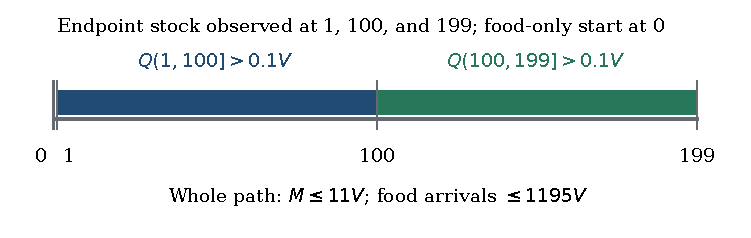
\includegraphics[width=.92\linewidth]{timeline.pdf}
\caption{The single-trajectory requirement. The endpoint stock condition is observed at the three marked times; the mass corridor and the arrival allowance cover the whole interval, including startup from the food-only state.}
\label{fig:timeline}
\end{figure}

Write $S_{a,n,V}=\PP(F_{n,V})$. The one-window event of the companion papers, $\Fold$, requires $M(t)\le11V$ for $0\le t\le100$ and $Q(1,100]>V/10$. Consequently
\begin{equation}\label{eq:inclusion}
 F_{n,V}\subseteq\Fold ,
\end{equation}
and this exact inclusion is the route by which every inherited converse estimate transfers.

\begin{lemma}[Material identities]\label{lem:material}
Let $J(t)$ be the signed change of nonfood monomer mass produced by all internal reactions up to time $t$, counting reverse reactions with their actual sign. Then for every trajectory and every $t\ge0$,
\begin{equation}\label{eq:balance}
 M_\nf(t)+Q(0,t]=M_\nf(0)+J(t)=J(t),\qquad 10V+B(t)\ \text{is the total monomer supplied by time }t .
\end{equation}
On $F_{n,V}$, therefore, $J(199)>V/5$ and
\begin{equation}\label{eq:yield}
 \frac{Q(0,199]}{10V+B(199)}>\frac{V/5}{10V+2\cdot1195V}=\frac1{12000}.
\end{equation}
\end{lemma}
\begin{proof}
Every jump changes $M_\nf$ by one of three amounts: a food arrival by zero, since foods carry no nonfood mass; a nonfood washout by exactly minus its export weight, which is what $Q$ accumulates; and an internal reaction by its signed nonfood mass change, which is what $J$ accumulates. Summing over the finitely many jumps on $[0,t]$ gives \eqref{eq:balance}, and $M_\nf(0)=0$ by the preparation. The supplied monomer is the initial mass $10V$ plus the arrivals $B(t)$. On the event the two windows export more than $V/5$ in total, the inventory $M_\nf(199)$ and the startup export $Q(0,1]$ are nonnegative, so $J(199)>V/5$; and $B(199)\le2A(199)\le2390V$ gives \eqref{eq:yield}.
\end{proof}

The fraction $1/12000\approx0.0083\%$ has monomer equivalents in numerator and denominator. It is a conservative material-recovery statement and not an energy efficiency, a purified yield, or a claim about the function of any exported species. Its content is that the export cannot be explained by preloaded nonfood inventory: there is none.

\section{Main results}\label{sec:main}

Fix the split identity $r_*=(00,11,0011)$ and let $A_n$ be the source event that all six food rows are empty and $r_*\in C_{0011}$; the other entries of the row $C_{0011}$ and all other nonfood rows are unrestricted. Row independence and exchangeability within a row give
\begin{equation}\label{eq:witness}
 \mu_{a,n}(A_n)=e_a^6\,p_{a,n}.
\end{equation}
Put
\begin{equation}\label{eq:constants}
 d=\frac1{6\times10^{20}},\qquad c=\frac{d^2}{8\times10^7}\approx3.47\times10^{-50},\qquad
 \delta_{n,V}=24e^{-cV/n},\qquad V_*(n)=10^{60}(n+1)^2 .
\end{equation}
A \emph{productive incidence} is a pair $(r,z)$ with $r=(u,v,uv)$, $u,v\in\cF$, $|uv|>2$, and $z\in\cF\cup\{uv\}$; $T_n$ is the event that some productive incidence is assigned. Let $K_*=10^{12}$ and let $L_n$ count the assigned incidences whose catalyst has length at most $K_*$ and whose product has length at most $K_*+2$; this \emph{$K_*$-rectangle} is finite and independent of $n$ and is never enumerated. With $c_{\rm old}=d^2/(4\times10^7)=2c$ define the residual
\begin{equation}\label{eq:residual}
 \bar r_{a,n,V}=\PP_{a,n}(L_n\ge2)+8e^{-c_{\rm old}V/n}.
\end{equation}

\begin{theorem}[Two consecutive windows]\label{thm:finite}
For every $n\ge4$, every $a>1$ and every integer $V\ge V_*(n)$:
\begin{align}
 \PP_\omega(F_{n,V})&\ge1-\delta_{n,V}\qquad\text{for every }\omega\in A_n\text{ and every mark configuration,}\label{eq:uniform}\\
 0<e_a^6p_{a,n}(1-\delta_{n,V})&\le\PP(F_{n,V}\cap A_n)\le S_{a,n,V},\label{eq:lower}\\
 S_{a,n,V}&\le\min\{1,\ 224p_{a,n}+\bar r_{a,n,V}\},\label{eq:upper}\\
 \PP(F_{n,V}\cap T_n^c)&\le\bar r_{a,n,V}.\label{eq:bad}
\end{align}
On $F_{n,V}$ the net internal nonfood synthesis through time $199$ exceeds $V/5$, and $Q(0,199]/(10V+B(199))>1/12000$.
\end{theorem}

The formal root uses the containing-rectangle coefficient $15480=30\cdot516$ in place of $224$; the census in Section~\ref{sec:converse} sharpens it. The uniform bound \eqref{eq:uniform} is what makes the theorem constructive: it holds pointwise for every environment in $A_n$, however many assignments the nonfood rows carry.

Now let $a_n=2-2/n$, let $V_n\ge V_*(n)$ be any integer sequence, and write $S_n=S_{a_n,n,V_n}$, $\bar r_n=\bar r_{a_n,n,V_n}$ and $\gamma=(6/\pi^2)^6$.

\begin{theorem}[Rarity and conditioning along the critical sequence]\label{thm:limits}
Along every such sequence,
\begin{align}
 \gamma\le\liminf_n\frac{S_n}{p_n}&\le\limsup_n\frac{S_n}{p_n}\le224,\label{eq:limbounds}\\
 \liminf_n\PP(A_n\mid F_{n,V_n})&\ge\frac\gamma{224},\qquad \PP(T_n^c\mid F_{n,V_n})\to0,\label{eq:posterior}\\
 2^np_n&\to\frac9{2\pi^2},\qquad S_n=\Theta(2^{-n}).\label{eq:rarity}
\end{align}
Numerically $\gamma\approx0.0504788$ and $\gamma/224\approx2.2535\times10^{-4}$.
\end{theorem}

The posterior statement is a liminf bound: it proves a positive asymptotic contribution of the constructed class, not that this class accounts for most successful reactors, and no exact limit of $S_n/p_n$ or of the posterior is asserted.

\begin{theorem}[Stopped first-birth ceiling]\label{thm:birth}
Let $\tau$ be the first time a nonfood molecule exists and $\sigma$ the first time $M>11V$. For $n\ge4$, food-only preparation, empty food rows, and every mark configuration, for every $t\ge0$,
\begin{equation}\label{eq:birth}
 \PP_\omega(\tau\le t,\ \tau<\sigma)\le1-e^{-\lambda Vt},\qquad\lambda=\frac{484}3\eps\approx3.2267\times10^{-7},
\end{equation}
and consequently $\PP_\omega(F_{n,V})\le1-e^{-\lambda V}$. Reliability $q(\omega)\ge1-\eta$, $0<\eta<1$, therefore requires $V\ge\log(1/\eta)/\lambda$; at $\eta=0.01$ this is $V\ge14\,272\,222$.
\end{theorem}

\begin{theorem}[Robustness in the Zipf exponent]\label{thm:robust}
Let $V_n\ge V_*(n)$ be any integer sequence and write $S_{a,n}=S_{a,n,V_n}$.
\begin{enumerate}[label=\textup{(\alph*)}]
\item\label{it:orders} \textup{(Exact orders.)} As $n\to\infty$, with $R=R_n\sim2n2^n$,
\begin{equation}\label{eq:orders}
 p_{a,n}\sim\begin{cases}
 \dfrac{R^{1-a}}{(a-1)(2-a)\zeta(a)},&1<a<2,\\[10pt]
 \dfrac{\log R}{\zeta(2)R},&a=2,\\[8pt]
 \dfrac{\zeta(a-1)/\zeta(a)-1}{R},&a>2,
 \end{cases}
 \qquad\text{so}\qquad
 p_{a,n}=\begin{cases}\Theta(n^{1-a}2^{-(a-1)n}),\\ \Theta(2^{-n}),\\ \Theta(n^{-1}2^{-n}).\end{cases}
\end{equation}
In particular $2^np_{2,n}\to3\log2/\pi^2$.
\item\label{it:order} \textup{(Rarity order for every exponent.)} For every fixed $a>1$, $S_{a,n}=\Theta(p_{a,n})$, with $\liminf S_{a,n}/p_{a,n}\ge\zeta(a)^{-6}$; the population of environments with $q(\omega)\ge1-\eta$ is also $\Theta(p_{a,n})$ for every fixed $\eta\in(0,1)$.
\item\label{it:dominance} \textup{(Singleton dominance for $a\ge2$.)} For every fixed $a\ge2$, $\PP(L_n\ge2)=o(p_{a,n})$; hence $\bar r_{a,n,V_n}/p_{a,n}\to0$, $\limsup S_{a,n}/p_{a,n}\le224$, $\PP(T_n^c\mid F_{n,V_n})\to0$ and $\liminf\PP(A_n\mid F_{n,V_n})\ge\zeta(a)^{-6}/224$.
\item\label{it:boundary} \textup{(The boundary $1<a<2$.)} For fixed $1<a<2$, $q_{2,a,n}/p_{a,n}\to2(2-a)/(3-a)>0$ and $\PP(L_n\ge2)\ge q_{2,a,n}$, so $\bar r_{a,n,V_n}=\Theta(p_{a,n})$: the residual of Theorem~\ref{thm:finite} is of the same order as the success probability and the conclusions of \ref{it:dominance} do not follow from it.
\item\label{it:family} \textup{(Critical families.)} For fixed real $\beta$ and $a_n=2-\beta/n$,
\begin{equation}\label{eq:family}
 2^np_{a_n,n}\to C(\beta)=\frac{3(2^\beta-1)}{\beta\pi^2}\ (\beta\ne0),\qquad C(0)=\frac{3\log2}{\pi^2},\qquad
 \frac{q_{2,a_n,n}}{p_{a_n,n}}\sim\frac{2\beta2^\beta}{n(2^\beta-1)}\to0,
\end{equation}
with $2/(n\log2)$ in place of the last expression at $\beta=0$, and every conclusion of \ref{it:dominance} holds along the family with lower prefactor $(6/\pi^2)^6$.
\end{enumerate}
\end{theorem}

Part \ref{it:family} at $\beta=2$ is Theorem~\ref{thm:limits}; the point of the theorem is that the exponential rarity scale $2^{-n}$ is shared by $a=2$ and by every critical family, that the rarity order survives for every exponent, and that heavier tails fail the converse for an identifiable reason, not by accident of the constants.

\begin{proposition}[Explicit witness reliability scales]\label{prop:scales}
Let $\omega\in A_n$ with any mark configuration and $0<\eta<1$.
\begin{enumerate}[label=\textup{(\alph*)}]
\item\label{it:direct} If $V\ge\max\{2n/d,\ (n/c)\log(24/\eta)\}$ then $q(\omega)\ge1-\eta$. At $\eta=0.01$ the second term is $2.2416\times10^{50}\,n$, which is $8.966\times10^{50}$ at $n=4$, against $2.5\times10^{61}$ under the envelope $V_*(4)$.
\item\label{it:unequal} Choosing the six noise tolerances of Appendix~\ref{app:constants} separately, at $99\%$ of their permitted limits, the condition
\begin{equation}\label{eq:unequal}
 V\ge\max\bigl\{5.001\times10^{49},\ 8.9\times10^{11}\,n\bigr\}
\end{equation}
implies $q(\omega)\ge0.99$. At $n=4$ this is about eighteen times smaller than \ref{it:direct}, the dominant term no longer depends on $n$, and it is set entirely by the absolute tolerance $\floorstock/100$ on the selected product coordinate.
\end{enumerate}
\end{proposition}

Both scales are pointwise reliability statements for the witness class; neither weakens the hypotheses of the converse or of the asymptotic theorems, and neither is a reactor design. The gap between \eqref{eq:unequal} and the necessary scale of Theorem~\ref{thm:birth} is $42$ orders of magnitude; Section~\ref{sec:scales} explains which tolerance is responsible and what a better estimate would have to do.

\section{Proof of the finite theorem}\label{sec:proof}

We separate the source-independent trajectory argument, valid pointwise on $A_n$, from source averaging and from the converse. Throughout this section $\omega\in A_n$, the marks are arbitrary, and $x_z=N_z/V$ denotes a normalized count; $u=x_{00}$, $w=x_{11}$, $x=x_{0011}$, $m=M_\nf/V$ and $L=M/V$.

\subsection{Loss envelopes from the generator}\label{sec:envelopes}
The following derivation produces the constants $23$ and $25$ directly from the propensities \eqref{eq:propensity}; it is the source of the drift inequalities that the companion paper \cite{structural2026} states.

\begin{lemma}[Loss envelopes]\label{lem:envelopes}
On $A_n$ and on the corridor $L\le11$, the coordinate drifts $b_u$, $b_w$, $b_x$ of the count process, evaluated at any state and divided by $V$, satisfy
\begin{equation}\label{eq:drifts}
 b_u\ge1-u-23Cu,\qquad b_w\ge1-w-23Cw,\qquad b_x\ge\eps uw+x(4uw-1-25C),\qquad
 C=4\eps+\tfrac{16}3m .
\end{equation}
\end{lemma}
\begin{proof}
On $A_n$ every food row is empty, so every active catalyst is nonfood and has length at least three; hence $\sum_{z\notin\cF}x_z\le m/3$. For any channel $r$, its basal coefficient is at most $4\eps$ and each catalytic coefficient is at most $16$, so the total coefficient of the channel, basal plus catalytic contributions weighted by catalyst concentration, is at most $4\eps+16\sum_{z\notin\cF}x_z\le C$. Falling factorials are bounded by powers, so the same envelope bounds every count propensity in which the channel appears, including the cases where the catalyst coincides with a substrate.

A species $y$ of normalized concentration $y$ is consumed by ligation in either ordered input position: for each partner $z$ and each of the two orderings the loss propensity over $V$ is at most $Cyx_z$, and the total over partners is at most $2Cy\sum_zx_z\le22Cy$, since $\sum_zx_z\le L\le11$. This count includes ligations of two identical copies, which remove two copies at a propensity bounded by $Cy^2$, and it includes the selected channel when $y$ is one of its substrates. Appearances as a catalyst do not consume the species. Cleavage of $y$ removes it at one split position for a dimer and at three positions for a length-four word, at rate at most $Cy$ and $3Cy$ respectively, and this includes the catalyzed reverse of the selected channel, whose catalyst $0011$ is nonfood and therefore already inside $C$. Adding the feed rate $1$ and the washout $-y$, and discarding every gain from internal reactions, gives $b_u\ge1-u-(22+1)Cu$, the same for $w$, and $b_x\ge-x-(22+3)Cx$ plus the retained gains. For $x$ we keep two gains: the basal forward firing of $r_*$, whose reactants $00$ and $11$ are distinct so its propensity over $V$ is exactly $b_{r_*}uw\ge\eps uw$, and the self-catalyzed forward firing $00+11+0011\to2\cdot0011$, with three distinct inputs and propensity over $V$ exactly $k_{r_*,0011}uwx\ge4uwx$.
\end{proof}

These are envelopes for the full catalogue, not equations for a closed three-species system: arbitrary nonfood background enters only through $m$, and the corridor bounds its aggregate catalytic influence. On the corridor $C<59$, which gives the crude startup bounds $b_u\ge1-1358u$, $b_w\ge1-1358w$ and $b_x\ge\eps uw-1476x$ used in Lemma~\ref{lem:startup}.

\subsection{The potential}\label{sec:potential}
Let $h(s)=(1-s)_+^2$, $H=h(u)+h(w)$, and
\begin{equation}\label{eq:potential}
 \Phi(u,w,x)=\log x-4H .
\end{equation}

\begin{lemma}[Drift of the potential]\label{lem:potential}
Let $(u,w,x)$ be differentiable with $u,w\ge0$, $x>0$, and derivatives satisfying \eqref{eq:drifts} at some $m\ge0$. Then
\begin{equation}\label{eq:phidot}
 \dot\Phi\ge2-117C=2-468\eps-624m .
\end{equation}
\end{lemma}
\begin{proof}
Put $\alpha=(1-u)_+$ and $\beta=(1-w)_+$. Since $u\ge1-\alpha\ge0$ and $w\ge1-\beta\ge0$, $uw\ge(1-\alpha)(1-\beta)\ge1-\alpha-\beta$, and $\alpha\le2\alpha^2+\tfrac18$ because $2(\alpha-\tfrac14)^2\ge0$; hence $uw\ge\tfrac34-2H$. Where $u<1$, $\frac d{dt}h(u)=-2\alpha\dot u\le-2\alpha(1-u-23Cu)=-2\alpha^2+46Cu\alpha\le-2h(u)+\tfrac{23}2C$, using $u\alpha=u(1-u)\le\tfrac14$; where $u\ge1$ the derivative of $h(u)$ is zero and the same bound holds. Thus $\dot H\le-2H+23C$. Discarding the nonnegative basal term in $b_x/x$,
\[
 \dot\Phi=\frac{\dot x}x-4\dot H\ge4uw-1-25C+8H-92C\ge3-1-117C .\qedhere
\]
\end{proof}

\begin{remark}[A sharper elementary inequality]\label{rem:fourfifths}
The inequality $uw\ge\tfrac34-2H$ can be replaced by $uw\ge\tfrac45-2H$: with $\alpha,\beta$ as above,
\[
 (1-\alpha)(1-\beta)+2(\alpha^2+\beta^2)-\tfrac45=\tfrac54\bigl(\alpha+\beta-\tfrac25\bigr)^2+\tfrac34(\alpha-\beta)^2\ge0,
\]
with equality at $u=w=\tfrac45$, so $\dot\Phi\ge\tfrac{11}5-117C$. This is a genuine improvement of \eqref{eq:phidot}, but the compensated estimate below uses perturbed constants that were established for the weaker bound, and we do not re-derive them here. The improvement would shorten the minimal window length (Section~\ref{sec:scales}) but does nothing for the count scale, which is set by a tolerance and not by the drift.
\end{remark}

\subsection{The count process: compensated coordinates and the interval telescope}\label{sec:count}
The jump process has holding intervals $[t_k,t_{k+1})$ on which the state $N^{(k)}$ is constant. For a coordinate $y$ write its compensator path $\tilde y(t)=y(0)+\int_0^tb_y(N(s))\dd s$, a continuous piecewise-linear function whose slope on the $k$-th holding interval is the drift $b_y(N^{(k)})$, and its noise $y(t)-\tilde y(t)$, a martingale. The \emph{corrected potential} $\Phi_\corr(t)=\Phi(\tilde u(t),\tilde w(t),\tilde x(t))$ is evaluated along the compensator paths, so it is continuous across jumps and differentiable inside holding intervals. A \emph{coordinate noise bound} with tolerance $\eta$ on horizon $T$ is the statement that $|y(t)-\tilde y(t)|\le\eta$ for all $t<T$ up to the first exit from the corridor; a \emph{mass noise bound} and \emph{reward noise bounds} for the export and gross-feed counters are defined in the same way, with the reward compensators $\int m\dd t$ and $6t$. The tolerances used are
\begin{equation}\label{eq:tolerances}
 \eta_M=\tfrac14,\qquad \eta_F=10^{-5}\ (u,w),\qquad \eta_P=\frac1{3\times10^{20}}\ (x),\qquad \eta_E=\tfrac1{40}\ (Q/V),\qquad \eta_B=1\ (A/V).
\end{equation}
The product tolerance is one percent of the stock floor $\floorstock$; this ratio, not the drift constants, is what later sets the count scale.

\begin{lemma}[Mass localization]\label{lem:mass}
From the food-only state, on the mass noise bound with tolerance $\tfrac14$ on horizon $T=200$, $M(t)\le11V$ for all $t<200$, and $M(t)\le\tfrac{21}2V$ at the three observation times.
\end{lemma}
\begin{proof}
The mass drift is $b_M/V=10-L$, so $\tilde L(t)=10$ for all $t$ from $L(0)=10$, and $|L-\tilde L|\le\tfrac14$ gives $L\le10.25$. The tolerance $\tfrac14$ is composed from a nonfood-mass tolerance $\tfrac18$ and a tolerance $\tfrac1{80}$ on each of the six food coordinates, whose mass weights sum to $10$; this composition is the origin of the coefficients $2$ and $12$ in the first two terms of \eqref{eq:six}.
\end{proof}

\begin{lemma}[Startup floor]\label{lem:startup}
Let $\omega\in A_n$ with any marks, start from the food-only state, and suppose that on horizon $T\le200$ the mass noise bound and the three coordinate noise bounds \eqref{eq:tolerances} for $u$, $w$ and $x$ hold. Then at every time $1\le t<T$,
\begin{equation}\label{eq:floor}
 u,w\ge\frac1{1358}-2\times10^{-5},\qquad x\ge\floorstock .
\end{equation}
\end{lemma}
\begin{proof}[Proof sketch; the checked statement is \lean{physical_startup_product_from_noise}]
By Lemma~\ref{lem:mass} the corridor holds on the horizon, so the crude bounds $b_u\ge1-1358u$ apply on every holding interval. The compensator $\tilde u$ then satisfies $\tilde u(t)\ge\tfrac1{1358}$ for all $t$ from $\tilde u(0)=1$, and the noise bound transfers this to $u$ up to $\eta_F$; the same holds for $w$. With $u,w\ge\tfrac1{1358}-2\cdot10^{-5}$, the product drift satisfies $b_x\ge\eps uw-1476x\ge6.9\times10^{-19}-1476x$, so $\tilde x(t)\ge\frac{6.9\times10^{-19}}{1476}(1-e^{-1476t})$, which exceeds $2\cdot\floorstock$ at $t=1$ and remains above it afterwards because the drift is positive below that level; the product noise $\eta_P$ is one percent of the floor.
\end{proof}

\begin{lemma}[Gain on a holding interval]\label{lem:holding}
Under the hypotheses of Lemma~\ref{lem:startup}, on a holding interval with state $N$ of mass at most $11V$ and $x\ge\floorstock$, for $0\le a\le b$ inside the interval and before $T$,
\begin{equation}\label{eq:holdgain}
 \Phi_\corr(b)-\Phi_\corr(a)\ge(b-a)\bigl(1.9-480\eps-640m(N)\bigr).
\end{equation}
\end{lemma}
\begin{proof}[Proof sketch; the checked statement is \lean{physical_holding_potential_gain}]
Inside the interval the compensator paths are linear with slopes given by the drifts at $N$, which satisfy \eqref{eq:drifts} in terms of the actual concentrations at $N$. The corrected coordinates differ from the actual ones by at most $\eta_F$, $\eta_F$ and $\eta_P$, and $\eta_P$ is at most one percent of $x$. Lemma~\ref{lem:potential} applied to the compensator paths with these perturbations, and with $\tfrac34-2H$ evaluated at the corrected foods, yields \eqref{eq:phidot} with the constants $2$, $468$, $624$ degraded to $1.9$, $480$, $640$.
\end{proof}

\begin{lemma}[Endpoint penalty]\label{lem:endpoint}
Under the same hypotheses, if $x\ge\floorstock$ at the two times $a\le b<T$ and the mass at time $b$ is at most $11V$, then $\Phi_\corr(b)-\Phi_\corr(a)<54$.
\end{lemma}
\begin{proof}
At time $b$, $4x\le L\le11$ gives $\tilde x\le\tfrac{11}4+\eta_P$ and $H\ge0$, so $\Phi_\corr(b)\le\log(\tfrac{11}4+\eta_P)<1.02$. At time $a$, $\tilde x\ge\floorstock-\eta_P$ and each corrected food is at least $-\eta_F$, so $H\le2(1+\eta_F)^2$ and $\Phi_\corr(a)>\log\bigl(0.99\cdot\floorstock\bigr)-8.0002>-50.56$. The difference is below $51.6$; the constant $54$ is the rounded value used in the checked statement \lean{physical_potential_endpoint_penalty}.
\end{proof}

\begin{proposition}[Interval occupation]\label{prop:interval}
Under the hypotheses of Lemma~\ref{lem:startup} with $T=200$, for every $1\le a\le b<200$,
\begin{equation}\label{eq:interval}
 \int_a^bm(t)\dd t\ge\frac{(b-a)(1.9-480\eps)-54}{640}.
\end{equation}
\end{proposition}
\begin{proof}
Let $J$ and $J+K$ index the holding intervals containing $a$ and $b$. By Lemma~\ref{lem:mass} the corridor holds up to time $b$, and by Lemma~\ref{lem:startup} the floor $x\ge\floorstock$ holds at every jump time in $[a,b]$ and at $a$ and $b$, since all these times are at least $1$. Apply Lemma~\ref{lem:holding} to the partial interval $[a,t_{J+1})$, to each full holding interval between, and to the partial interval $[t_{J+K},b]$; the corrected potential is continuous at jumps, so the increments telescope to $\Phi_\corr(b)-\Phi_\corr(a)$, while the right-hand sides sum to $(b-a)(1.9-480\eps)-640\int_a^bm\dd t$ because $m$ is constant on each holding interval. Lemma~\ref{lem:endpoint} bounds the left-hand side by $54$. The checked assembly is \lean{physical_interval_mass_from_noise}.
\end{proof}

This is the whole content of the extension from one window to two: the estimate is stated for an arbitrary actual interval of the same trajectory, with both partial holding intervals retained, and no new initial law is introduced at the middle observation time.

\begin{corollary}[Export in a window]\label{cor:export}
Under the hypotheses of Proposition~\ref{prop:interval} and the export reward noise bound with tolerance $\tfrac1{40}$,
\begin{equation}\label{eq:margin}
 \frac{Q(a,b]}V\ge\frac{(b-a)(1.9-480\eps)-54}{640}-\frac1{20},
\end{equation}
which for $b-a=99$ equals $0.1595311015>0.1$. The right-hand side exceeds $\tfrac1{10}$ exactly when $b-a\ge79$; a window of length $78$ does not satisfy the sufficient inequality.
\end{corollary}
\begin{proof}
The compensator of $Q/V$ is $\int m\dd t$, so $Q(a,b]/V$ differs from $\int_a^bm\dd t$ by the difference of two prefix noises, each at most $\tfrac1{40}$ (\lean{physical_interval_export_lower}). The numerical values are $\bigl(99(1.9-480\eps)-54\bigr)/640=0.2095311015$ and $150/(1.9-480\eps)=78.95$.
\end{proof}

Applied to $[1,100]$ and $[100,199]$ this gives both windows. Lemma~\ref{lem:startup} gives the stock floor at $1$, $100$ and $199$ and Lemma~\ref{lem:mass} the mass bound $\tfrac{21}2V$ there, so endpoint stock holds at all three times; the corridor holds through $199$; and the gross-feed compensator is exactly $6t$, so the reward noise bound with tolerance $1$ gives $A(199)/V\le6\cdot199+1=1195$. The event $F_{n,V}$ therefore holds on the intersection of the six noise bounds.

\subsection{One simultaneous probability estimate}\label{sec:noise}
\begin{lemma}[Six-term failure bound]\label{lem:six}
Let $\omega\in A_n$ with any marks and let $V$ be an integer. For every choice of positive tolerances $d_N,d_M,d_F,d_P,d_E,d_B$ with
\begin{equation}\label{eq:margins}
\begin{gathered}
 d_N+\frac nV\le\frac18,\qquad d_M+\frac2V\le\frac1{80},\qquad d_F+\frac2V\le10^{-5},\\
 d_P+\frac2V\le\frac1{3\times10^{20}},\qquad d_E+\frac nV\le\frac1{40},\qquad d_B+\frac nV\le1,
\end{gathered}
\end{equation}
the food-only trajectory law satisfies
\begin{align}
 \PP_\omega(F_{n,V}^c)&\le2e^{-E_N(d_N)}+12e^{-E_C(d_M)}+4e^{-E_C(d_F)}\notag\\
 &\qquad+2e^{-E_C(d_P)}+2e^{-E_N(d_E)}+2e^{-E_N(d_B)},\label{eq:six}
\end{align}
\begin{equation}\label{eq:exponents}
 E_N(s)=\frac{s^2V}{4n(96011\cdot200+s)},\qquad E_C(s)=\frac{s^2V}{4(96000\cdot200+2s)} .
\end{equation}
\end{lemma}
\begin{proof}
By Section~\ref{sec:count}, $F_{n,V}^c$ is contained in the union of the six noise-bound failures, and the union bound applies; no independence is used. Each failure probability is an exponential martingale tail bound of Freedman type \cite{freedman1975tail} for the compensated jump process stopped at corridor exit: the jump sizes of a normalized coordinate are at most $2/V$ and of the mass and reward counters at most $n/V$, the predictable quadratic variation on the horizon $200$ is bounded on the corridor by the total rate envelope $96000$ per unit time for a coordinate and $96011$ for the mass and rewards, and the margin conditions \eqref{eq:margins} absorb the jump-size correction so that a noise bound with the tolerance of \eqref{eq:tolerances} follows from the centred tail with parameter $d$. The twelve food terms arise from the composition in Lemma~\ref{lem:mass}. The checked statement is \lean{physical_two_window_failure_tail}, whose hypotheses are exactly: empty food rows, the selected incidence with distinct dimer inputs and length-four product, the coefficient bounds \eqref{eq:marks}, the food-only initial state, and \eqref{eq:margins}.
\end{proof}

Setting all six tolerances equal to $d$ and requiring $V\ge2n/d$ verifies \eqref{eq:margins} for $n\ge4$, and every exponent is then at least $cV/n$ because $4(96011\cdot200+d)\le8\times10^7$ and $4(96000\cdot200+2d)\le8\times10^7$; this gives $\PP_\omega(F_{n,V}^c)\le24e^{-cV/n}=\delta_{n,V}$, which is \eqref{eq:uniform} once $V\ge V_*(n)\ge2n/d$. The choice is convenient rather than optimal; Proposition~\ref{prop:scales}\ref{it:unequal} exploits the freedom. Under $V\ge V_*(n)$, $cV/n\ge48$ and $24e^{-48}<\tfrac12$, so the lower bound in \eqref{eq:lower} is positive.

\subsection{Source averaging}\label{sec:averaging}
The bound \eqref{eq:uniform} holds for every $\omega\in A_n$ and every mark configuration. Averaging first over the trajectory law, then over the uniform mark law, then over the source restricted to $A_n$, and using the exact mass \eqref{eq:witness}, gives $\PP(F_{n,V}\cap A_n)\ge e_a^6p_{a,n}(1-\delta_{n,V})$. The exact source mass is computed from the configuration weight without any approximation: the six food rows contribute $\PP(D=0)^6$ and the selected row contributes the probability that a uniformly random $D$-subset contains $r_*$, averaged over $D$, which is $\EE D/R_n$ (\lean{source_food_silent_seed_mass}). This proves \eqref{eq:lower}.

\subsection{The converse and the productive census}\label{sec:converse}
\begin{lemma}[Inherited one-window exclusion \cite{diffuse2026}]\label{lem:exclusion}
Let $\omega$ be an environment, with arbitrary marks and arbitrary assignments outside the $K_*$-rectangle, such that at most one incidence lies in the rectangle and no productive incidence is assigned. For every integer $V\ge2n/d$ with $n/V\le1/200000$, from the food-only state,
\begin{equation}\label{eq:exclusion}
 \PP_\omega(\Fold)\le4e^{-c_{\rm old}V/n}+2e^{-E'(1/200)}+2e^{-E'(1/200000)}\le8e^{-c_{\rm old}V/n},
 \qquad E'(s)=\frac{s^2V}{4n(96011\cdot101+s)} .
\end{equation}
\end{lemma}
The first inequality is \lean{physical_output_upper_at_most_one_local}; its mechanism is a conserved product credit that cancels a mixed food--nonfood channel exactly, and a washout penalty that lets the dilution of an outsider catalyst pay for the material it could amplify. The second inequality holds for all $n$ and $V$ because both extra exponents exceed $c_{\rm old}V/n$ by more than thirty orders of magnitude.

\begin{lemma}[Productive census]\label{lem:census}
For every $n\ge4$ there are exactly $224$ productive incidences: $32$ food-to-nonfood split identities, each with six food catalysts and its own product as the seventh, hence $192$ food-catalyzed and $32$ product-self-catalyzed labels. The event $T_n$ is exactly the union over these labels of the events $\{r\in C_z\}$, and
\begin{equation}\label{eq:census}
 \PP_{a,n}(T_n)\le224\,p_{a,n}.
\end{equation}
\end{lemma}
\begin{proof}
A productive identity has food inputs and nonfood product, so its product has length three or four: $2\cdot4=8$ monomer--dimer ordered pairs, $8$ dimer--monomer pairs, and $4\cdot4=16$ dimer--dimer pairs, in total $32$; the ordered convention counts $(0,01,001)$ and $(00,1,001)$ separately. For each identity the seven admissible catalysts are distinct choices, so there are $32\cdot7=224$ labels, all with catalyst length at most $4$ and product length at most $4$; the same short words occur in every catalogue with $n\ge4$, which proves the count for all $n$. The union bound \eqref{eq:census} uses only the common marginal $p_{a,n}$ and no independence. The cap-four count, the equivalence of the predicate with the union event, and an injection of the labels of every larger catalogue into those at cap four are checked in \lean{ProductiveCensus.lean}; the reverse inclusion is the sentence above.
\end{proof}

\begin{proof}[Proof of \eqref{eq:upper} and \eqref{eq:bad}]
By \eqref{eq:inclusion}, $\PP(F_{n,V}\cap T_n^c)\le\PP(\Fold\cap T_n^c)$. Split the environments in $T_n^c$ according to whether $L_n\ge2$. The first part has source probability $\PP_{a,n}(L_n\ge2)$; on the second, Lemma~\ref{lem:exclusion} applies, since $V\ge V_*(n)$ implies both of its scale hypotheses. This gives \eqref{eq:bad}, and $S_{a,n,V}\le\PP(T_n)+\PP(F_{n,V}\cap T_n^c)$ with Lemma~\ref{lem:census} gives \eqref{eq:upper}. The formal root proves the same inequalities with the containing rectangle of all catalysts of length at most $4$ and all identities of product length at most $6$, whose size is $30\cdot516=15480$.
\end{proof}

\subsection{The accounts}
The statements about net synthesis and the recovered fraction are Lemma~\ref{lem:material}; the pathwise identity \eqref{eq:balance} is \lean{actual_net_synthesis_identity} and the scalar inequality \eqref{eq:yield} is \lean{mission_material_recovery}. This completes the proof of Theorem~\ref{thm:finite}.

\section{Limits and consequences}\label{sec:consequences}

\subsection{Proof of Theorem~\ref{thm:limits}}
The inherited exact-source limits for the capped, shifted sampler at $a_n=2-2/n$ are
\begin{equation}\label{eq:sourcelimits}
 e_n\to\frac6{\pi^2},\qquad X_np_n\to\frac9{\pi^2},\qquad \frac{\bar r_n}{p_n}\to0,\qquad \delta_{n,V_n}\to0
\end{equation}
(\lean{collective_empty_row_limit}, \lean{sourceExactCriticalFirstMoment_scaled_tendsto}, \lean{mission_residual_relative_tendsto_zero}, \lean{two_window_noise_tendsto_zero}). The third uses the excess-count estimate of \cite{diffuse2026} for two incidences in a fixed rectangle, which retains the dependence within a row, together with $e^{-c_{\rm old}V_n/n}\le e^{-3n}=o(p_n)$. Dividing \eqref{eq:lower} and \eqref{eq:upper} by $p_n$ proves \eqref{eq:limbounds}. Next,
\begin{equation}\label{eq:posteriorfinite}
 \PP(A_n\mid F_{n,V_n})=\frac{\PP(F_{n,V_n}\cap A_n)}{S_n}\ge\frac{e_n^6(1-\delta_{n,V_n})}{224+\bar r_n/p_n},
\end{equation}
which gives the first part of \eqref{eq:posterior}; dividing \eqref{eq:bad} by the positive lower bound in \eqref{eq:lower} gives the second. Finally $X_n/2^n\to2$ gives \eqref{eq:rarity}. The formal root proves the eventual bounds with the coefficients $\gamma/2$ and $15481$ and the vanishing conditional probability of no productive singleton; the full constants are the conventional sharpening just given. \qed

\subsection{Screening}
For $N$ independent complete experiments, each with fresh chemistry, marks, preparation and clock, the probability of at least one success is $1-(1-S_n)^N$, and the least $N$ reaching confidence $\alpha$ is
\begin{equation}\label{eq:screen}
 N_\alpha=\Bigl\lceil\frac{\log(1-\alpha)}{\log(1-S_n)}\Bigr\rceil=\Theta(2^n),
\end{equation}
by $-\log(1-s)\sim s$ and \eqref{eq:rarity}. A finite lower bound on $S_n$ gives a sufficient trial count and a finite upper bound below one a necessary one. Repeating $N$ runs in one sampled environment is a different experiment: its success probability is the mixture $1-\EE_\mu[(1-q(\omega))^N]$, and replacing it by $1-(1-\EE_\mu q)^N$ is unjustified, because $q$ is far from constant across environments.

\subsection{Reliable environments}
If $0<\eta<1$ and $\delta_{n,V}\le\eta$, then
\begin{equation}\label{eq:reliable}
 e_a^6p_{a,n}\le\mu_{a,n}\{q\ge1-\eta\}\le\frac{S_{a,n,V}}{1-\eta}.
\end{equation}
The lower inclusion is \eqref{eq:uniform}; the upper bound integrates $q\ge(1-\eta)\ind_{\{q\ge1-\eta\}}$. Along the critical sequence the reliable population is therefore $\Theta(p_n)$ with liminf prefactor at least $\gamma$ and limsup at most $224/(1-\eta)$. The full law of the reliable population is not identified.

\subsection{Transfers that preserve the actual event}\label{sec:transfers}
If a source or path property $B_n$ satisfies $\PP(\Fold\cap B_n^c)=o(p_n)$, then by \eqref{eq:inclusion} and \eqref{eq:limbounds}
\begin{equation}\label{eq:transfer}
 \PP(B_n^c\mid F_{n,V_n})\le\frac{\PP(\Fold\cap B_n^c)}{S_n}\to0 .
\end{equation}
Four instances follow.

\emph{Unique productive incidence.} Every productive label lies in the $K_*$-rectangle, so two productive incidences force $L_n\ge2$, an event of source probability $o(p_n)$. Hence, conditional on success, exactly one productive incidence is present with probability tending to one. This says nothing about the relative frequencies of the $224$ labels.

\emph{Catalytic deletion.} Delete every catalytic channel while keeping the basal coefficients, preparation, feed and washout. The companion theorem \cite{structural2026} bounds the disabled success probability of $\Fold$ by $2e^{-c_{\rm old}V/n}$ in every environment; by \eqref{eq:inclusion} the same bounds $F_{n,V}$, and after averaging its ratio to $S_n$ tends to zero. Positive basal chemistry remains, so the disabled probability is not declared zero.

\emph{Nesting of the two events.} The census converse also bounds $\PP(\Fold)\le224p_n+\bar r_n$, so
\begin{equation}\label{eq:nesting}
 \liminf_n\PP(F_{n,V_n}\mid\Fold)\ge\frac\gamma{224}.
\end{equation}
The stronger task keeps the rarity order of the weaker one; this does not say that most first-window successes repeat.

\emph{Conditioning on structure.} Every productive label is a singleton RAF in the reversible convention, so $T_n\subseteq G_n$, the event that some RAF exists. The companion structural theorem gives $\PP(G_n)\to\theta>0$ as a genuine limit (\lean{source_RAF_probability_tendsto}, positive by \lean{sourceCriticalSurvival_pos}). Since $F_{n,V_n}\cap G_n^c\subseteq F_{n,V_n}\cap T_n^c$, \eqref{eq:bad} gives $\PP(F_{n,V_n}\cap G_n)=S_n-o(p_n)$, hence $\PP(F_{n,V_n}\mid G_n)=\Theta(p_n)$ and $\PP(F_{n,V_n}\mid G_n)/S_n\to\theta^{-1}$. No independent-incidence structural theorem is used.

\section{The necessary discrete startup scale}\label{sec:startup}

The concentration-level argument of Section~\ref{sec:proof} says nothing about initiation at small counts. The following bound applies to every food-silent environment and every mark configuration, without a limit in $n$ or $V$.

\begin{proof}[Proof of Theorem~\ref{thm:birth}]
Before $\tau$ every nonfood molecule has zero count and every food molecule has an empty row, so all catalytic propensities vanish and a first nonfood molecule can only be made by a basal ligation of two foods. Put $x=\sum_{|z|=1}x_z$ and $y=\sum_{|z|=2}x_z$. The ordered food pairs whose ligation is nonfood are monomer--dimer, dimer--monomer and dimer--dimer, with ordinary reactant-product sum $2xy+y^2$; falling factorials are bounded by powers, including for identical dimers, and each basal coefficient is at most $4\eps$. On the corridor $x+2y\le11$,
\begin{equation}\label{eq:hazard}
 \lambda_{\rm birth}(N)\le4\eps V(2xy+y^2)\le4\eps V(22y-3y^2)\le\frac{484}3\eps V=\lambda V,
\end{equation}
the maximum being at $y=\tfrac{11}3$, $x=\tfrac{11}3$ (\lean{food_pair_birth_bound}, \lean{startup_intensity_bound}).

Stop the process at $\tau\wedge\sigma$. Before either stopping event only finitely many population states are reachable. Send a corridor exit to a safe absorbing state and a first birth to a distinct absorbing failure state; a birth preserves total monomer mass, so it cannot coincide with a corridor exit. Uniformize the resulting finite chain at a rate $q$ at least its maximal total rate and at least $\lambda V$: the chain then moves at the ticks of a Poisson process of rate $q$, and in every nonfailure state the one-tick failure probability is at most $\lambda V/q$. By induction over ticks, conditional survival through $k$ ticks is at least $(1-\lambda V/q)^k$ whatever the intervening states (\lean{startup_survival_lower}). Averaging over the independent Poisson tick count,
\begin{equation}\label{eq:mixture}
 \sum_{k\ge0}e^{-qt}\frac{(qt)^k}{k!}\Bigl(1-\frac{\lambda V}q\Bigr)^k=e^{-\lambda Vt}.
\end{equation}
This is a domination argument; the state-dependent birth count itself is not Poisson. The stopped chain agrees with the original path until the first stopping event, which proves \eqref{eq:birth}. The event $F_{n,V}$ requires a length-four molecule at time $1$ and no corridor exit through $199$, so it is contained in $\{\tau\le1,\tau<\sigma\}$, and $\PP_\omega(F_{n,V})\le1-e^{-\lambda V}$ follows. Finally $1-\eta\le1-e^{-\lambda V}$ is equivalent to $\lambda V\ge\log(1/\eta)$ (\lean{startup_necessary_scale}), and $\log(100)/\lambda=14\,272\,221.65$.
\end{proof}

At $V=100$ the food-silent mission probability is at most $3.2266\times10^{-5}$, at $V=200$ at most $6.4531\times10^{-5}$, and a birth before time $199$ and before corridor exit has probability at most $0.0064$ at $V=100$. These are upper bounds and necessary conditions, not sufficient startup estimates: the first nonfood molecule need not be the selected product, a seed can wash out, and growth to operating stock is a further event. The restriction applies to food-silent environments, the coefficients \eqref{eq:marks}, the food-only preparation and the startup deadline $1$; a food-catalyzed productive incidence can initiate immediately, and changing $\eps$, the deadline or the preparation changes the question. Figure~\ref{fig:startup} shows the ceiling.

\begin{figure}[t]
\centering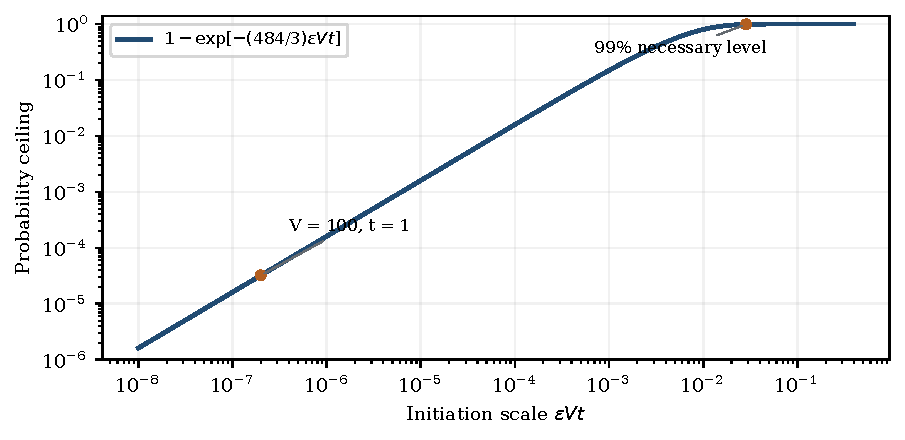
\includegraphics[width=.8\linewidth]{startup.pdf}
\caption{The first-birth ceiling $1-\exp[-(484/3)\eps Vt]$ as a function of $\eps Vt$. For the mission $t=1$, and the bound applies to every food-silent environment and every mark configuration. The marked $99\%$ level is a necessary initiation scale, not a sufficient operating design.}
\label{fig:startup}
\end{figure}

\section{Robustness in the Zipf exponent}\label{sec:robust}

The finite Theorem~\ref{thm:finite} holds for every $a>1$. This section computes how its constants scale and proves Theorem~\ref{thm:robust}; the first-moment limit along the families of part~\ref{it:family} is formally verified for every $\beta$ (\lean{windowZipfMean_source_window_normalized}), and everything else here is a conventional deduction.

\subsection{Exact moments and fixed-exponent asymptotics}
Write $T_R=\sum_{k\ge R}k^{-a}$ and $R=R_n$. From \eqref{eq:degreelaw},
\begin{equation}\label{eq:moments}
 \EE D=\frac{\sum_{k=1}^{R-1}k^{1-a}+RT_R}{\zeta(a)}-1,\qquad
 \EE[D(D-1)]=\frac{\sum_{k=1}^{R-1}(k-1)(k-2)k^{-a}+(R-1)(R-2)T_R}{\zeta(a)} .
\end{equation}
The first form follows from $\EE D=\zeta(a)^{-1}[\sum_{k<R}(k-1)k^{-a}+(R-1)T_R]$ by writing $(k-1)k^{-a}=k^{1-a}-k^{-a}$ and $\sum_{k<R}k^{-a}=\zeta(a)-T_R$. Both are evaluated without enumeration through Hurwitz zeta values.

\begin{proof}[Proof of Theorem~\ref{thm:robust}\ref{it:orders}]
For $0<s<1$, $\sum_{k<R}k^{-s}=R^{1-s}/(1-s)+O(1)$; for $s=1$ the sum is $\log R+O(1)$; for $s>1$ it converges to $\zeta(s)$; and $T_R=R^{1-a}/(a-1)+O(R^{-a})$. For $1<a<2$ the two growing terms of $\EE D$ are $R^{2-a}/(2-a)$ and $R^{2-a}/(a-1)$, whose sum is $R^{2-a}/[(a-1)(2-a)]$. For $a=2$ the finite sum is harmonic and $RT_R\to1$. For $a>2$ dominated convergence gives $\EE D\to\zeta(a-1)/\zeta(a)-1$. Dividing by $R\sim2n2^n$ gives \eqref{eq:orders}; at $a=2$, $\log R\sim n\log2$ and $2^np_{2,n}\to\log2/(2\zeta(2))=3\log2/\pi^2$.
\end{proof}

Figure~\ref{fig:exponent} shows the exact values of $2^np_{a,n}$ for several exponents; Table~\ref{tab:orders} summarizes the orders.

\begin{table}[t]
\centering\footnotesize\setlength{\tabcolsep}{4pt}
\begin{tabular}{@{}llll@{}}
\toprule
Exponent & $p_{a,n}$ & $q_{2,a,n}/p_{a,n}$ & singleton dominance, limiting prefactors\\
\midrule
$1<a<2$ & $\Theta(n^{1-a}2^{-(a-1)n})$ & $\to2(2-a)/(3-a)>0$ & not by the present converse\\
$a=2$ & $\Theta(2^{-n})$, $2^np\to3\log2/\pi^2$ & $\sim2/\log R\to0$ & yes, $[\zeta(2)^{-6},224]$\\
$a_n=2-\beta/n$ & $\Theta(2^{-n})$, $2^np\to C(\beta)$ & $\sim2\beta2^\beta/[n(2^\beta-1)]\to0$ & yes, $[(6/\pi^2)^6,224]$\\
$a>2$ & $\Theta(n^{-1}2^{-n})$ & $O(R^{2-a}\log R)\to0$ & yes, $[\zeta(a)^{-6},224]$\\
\bottomrule
\end{tabular}
\caption{Orders of the incidence probability and of the same-row pair ratio, and the status of singleton dominance, for the volume sequence $V_n\ge V_*(n)$ (Theorem~\ref{thm:robust}). In every row the success probability is $\Theta(p_{a,n})$.}
\label{tab:orders}
\end{table}

\begin{figure}[t]
\centering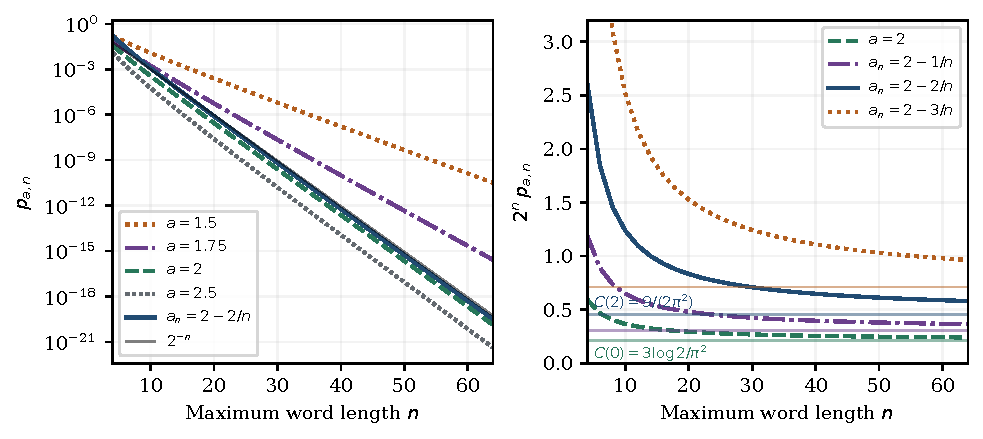
\includegraphics[width=.98\linewidth]{exponent.pdf}
\caption{Exact incidence probabilities from \eqref{eq:moments}. Left: $p_{a,n}$ for fixed exponents and for $a_n=2-2/n$ against $2^{-n}$; the rarity exponent is $(a-1)\log2$ below $a=2$ and $\log2$ at and above it. Right: $2^np_{a,n}$ for $a=2$ and for the families $a_n=2-\beta/n$, $\beta=1,2,3$, with the limits $C(\beta)$ of \eqref{eq:family} as horizontal lines; the approach is of relative order $1/n$. The curves are source moments, not success probabilities.}
\label{fig:exponent}
\end{figure}

\subsection{The rarity order for every exponent}
\begin{proof}[Proof of Theorem~\ref{thm:robust}\ref{it:order}]
Let $H_K=(2^{K+1}-2)(K2^{K+3}+4)$ with $K=K_*$: the number of catalyst--identity pairs in the full $K_*$-rectangle, an enormous but fixed constant. Since $L_n$ is a sum of at most $H_K$ indicators of common marginal $p_{a,n}$, Markov's inequality gives $\PP(L_n\ge2)\le\tfrac12\EE L_n\le\tfrac12H_Kp_{a,n}$, without any independence. Theorem~\ref{thm:finite} then gives, for $V_n\ge V_*(n)$,
\begin{equation}\label{eq:robustsandwich}
 \tfrac12e_a^6p_{a,n}\le S_{a,n}\le\bigl(224+\tfrac12H_K\bigr)p_{a,n}+8e^{-c_{\rm old}V_n/n},
\end{equation}
using $\delta_{n,V_n}\le\tfrac12$. Under the envelope, $c_{\rm old}V_n/n\ge3n$, so the last term is at most $8e^{-3n}$, which is $o(p_{a,n})$ in every case of \eqref{eq:orders} because $(a-1)\log2<3$. Hence $S_{a,n}=\Theta(p_{a,n})$, with $\liminf S_{a,n}/p_{a,n}\ge\zeta(a)^{-6}$ since $\delta_{n,V_n}\to0$. The reliable-population statement is \eqref{eq:reliable}, valid once $\delta_{n,V_n}\le\eta$.
\end{proof}

The implied upper constant in \eqref{eq:robustsandwich} is useless as a finite number; the content of the statement is that the source-to-operation comparison, success of order the incidence probability, survives for every exponent while the exponent itself changes in the computable way \eqref{eq:orders}.

\subsection{Second moments: dominance for \texorpdfstring{$a\ge2$}{a >= 2} and the boundary}
\begin{proof}[Proof of Theorem~\ref{thm:robust}\ref{it:dominance} and \ref{it:boundary}]
Two distinct incidences in the rectangle either share a catalyst, with joint probability $q_{2,a,n}$, or lie in different rows, with joint probability $p_{a,n}^2$; a union bound over the fixed rectangle gives
\begin{equation}\label{eq:pairs}
 \PP(L_n\ge2)\le C_{\rm same}q_{2,a,n}+C_{\rm diff}p_{a,n}^2
\end{equation}
with constants depending only on the rectangle. From \eqref{eq:moments}, expanding $(k-1)(k-2)=k^2-3k+2$: for $1<a<2$ the growing terms of $\EE[D(D-1)]$ are $R^{3-a}/(3-a)$ from the sum and $R^{3-a}/(a-1)$ from the atom, so
\[
 q_{2,a,n}\sim\frac{2R^{1-a}}{(a-1)(3-a)\zeta(a)},\qquad\frac{q_{2,a,n}}{p_{a,n}}\to\frac{2(2-a)}{3-a};
\]
for $a=2$ both terms are $\sim R$, so $q_{2,2,n}\sim2/(\zeta(2)R)$ and $q_2/p\sim2/\log R\to0$; for $a>2$ the numerator grows at most like $R^{3-a}$, $\log R$ or $O(1)$, so $q_2/p=O(R^{2-a}\log R)\to0$. In every case $p_{a,n}\to0$. Hence for $a\ge2$ the right-hand side of \eqref{eq:pairs} is $o(p_{a,n})$, so $\bar r_{a,n,V_n}/p_{a,n}\to0$, and the arguments of Section~\ref{sec:consequences} apply verbatim with $e_a=\zeta(a)^{-1}$ in place of $e_n$: this is \ref{it:dominance}. For $1<a<2$, $\PP(L_n\ge2)\ge q_{2,a,n}$ because two fixed productive labels with a common catalyst lie in the rectangle, and $q_{2,a,n}=\Theta(p_{a,n})$ by the limit just computed: this is \ref{it:boundary}.
\end{proof}

Part \ref{it:boundary} is a substantive boundary rather than a technical inconvenience. For a heavy-tailed row, conditioning on one required incidence leaves a nonvanishing probability of a second prescribed incidence in the same row, so a successful incidence typically arrives with a substantial local catalytic background, and a converse must weigh that background dynamically rather than exclude it by counting. This does not prove that singleton dominance fails after conditioning on successful dynamics for $1<a<2$; it identifies the additional estimate that would be needed.

\subsection{Critical families}
\begin{proof}[Proof of Theorem~\ref{thm:robust}\ref{it:family}]
Along $a_n=2-\beta/n$, $\log R/n\to\log2$ and $R^{\beta/n}\to2^\beta$. In \eqref{eq:moments}, $\sum_{k<R}k^{-1+\beta/n}=n(R^{\beta/n}-1)/\beta+O(1)\sim n(2^\beta-1)/\beta$ for $\beta\ne0$ and $\sim n\log2$ for $\beta=0$, while $RT_R\to2^\beta$ is bounded; so $\EE D\sim n(2^\beta-1)/(\beta\zeta(2))$, and dividing by $R\sim2n2^n$ gives $C(\beta)$, with $C(0)$ by continuity. This limit is the formally verified statement that $\EE D/n\to(1-2^{-b})/(b\zeta(2))$ at exponent $2+b/n$, with $b=-\beta$. For the second moment, $\sum_{k<R}k^{\beta/n}\sim R\,2^\beta$ and $R^2T_R\sim R\,2^\beta$, so $\EE[D(D-1)]\sim2\cdot2^\beta R/\zeta(2)$ and
\[
 \frac{q_{2,a_n,n}}{p_{a_n,n}}\sim\frac{2\cdot2^\beta/(\zeta(2)R)}{n(2^\beta-1)/(\beta\zeta(2)R)}=\frac{2\beta2^\beta}{n(2^\beta-1)}\to0,
\]
and $2/(n\log2)$ at $\beta=0$. The rest is \eqref{eq:pairs} and Section~\ref{sec:consequences}, with $e_{a_n}\to6/\pi^2$ for every $\beta$. The moment estimates are established directly along the sequence from the capped sums; fixed-exponent asymptotics are not invoked as if they were uniform.
\end{proof}

\section{Explicit scales and the converse obstruction}\label{sec:scales}

\subsection{Proof of Proposition~\ref{prop:scales}}
\ref{it:direct} The uniform bound $\PP_\omega(F_{n,V}^c)\le24e^{-cV/n}$ was proved in Section~\ref{sec:noise} under $V\ge2n/d$ alone, so $24e^{-cV/n}\le\eta$, that is $V\ge(n/c)\log(24/\eta)$, suffices. Numerically $\log(2400)/c=2.2416\times10^{50}$.

\ref{it:unequal} Take $(d_N,d_M,d_F,d_P,d_E,d_B)=0.99\cdot(\tfrac18,\tfrac1{80},10^{-5},\tfrac1{3\times10^{20}},\tfrac1{40},1)$. The margins \eqref{eq:margins} then hold exactly when $V\ge\max\{800n,16000,2\times10^7,6\times10^{22},4000n,100n\}$. Allocating $\eta/6$ to each term of \eqref{eq:six}, a term $b\,e^{-E_N(s)}$ is at most $\eta/6$ once $V\ge4n(96011\cdot200+s)s^{-2}\log(6b/\eta)$, and similarly with $4(96000\cdot200+2s)$ for an $E_C$ term. At $\eta=0.01$ the six thresholds are listed in Table~\ref{tab:unequal}; rounding upward gives \eqref{eq:unequal}, and the ratio of $8.966\times10^{50}$ to $5.0002\times10^{49}$ is $17.9$. The product term has no factor $n$ because the coordinate exponent $E_C$ has none; replacing all six exponents by the common $cV/n$ introduces that dependence needlessly. Lemma~\ref{lem:six} admits independent tolerances in exactly this form, so no hidden common-tolerance premise is used. \qed

\begin{table}[t]
\centering\small
\begin{tabular}{@{}llrr@{}}
\toprule
Term of \eqref{eq:six} & tolerance & sufficient $V$ at $\eta=0.01$ & deterministic margin\\
\midrule
$2e^{-E_N(d_N)}$ (nonfood mass) & $0.99/8$ & $3.556\times10^{10}\,n$ & $800n$\\
$12e^{-E_C(d_M)}$ (six foods, mass) & $0.99/80$ & $4.454\times10^{12}$ & $16000$\\
$4e^{-E_C(d_F)}$ (selected foods) & $0.99\times10^{-5}$ & $6.099\times10^{18}$ & $2\times10^7$\\
$2e^{-E_C(d_P)}$ (selected product) & $0.99/(3\times10^{20})$ & $5.000\times10^{49}$ & $6\times10^{22}$\\
$2e^{-E_N(d_E)}$ (export) & $0.99/40$ & $8.890\times10^{11}\,n$ & $4000n$\\
$2e^{-E_N(d_B)}$ (gross feed) & $0.99$ & $5.556\times10^{8}\,n$ & $100n$\\
\bottomrule
\end{tabular}
\caption{Unequal-tolerance evaluation of the six-term bound at $99\%$ witness reliability. The product term dominates by thirty orders of magnitude; the $n$-dependent terms would take over only beyond $n\approx5.6\times10^{37}$.}
\label{tab:unequal}
\end{table}

\subsection{What sets the scale}
Three quantities restrict the count scale: the jump correction $n/V\le d/2$, which needs $V\ge1.2\times10^{21}n$; the exponential suppression needed for a stated reliability, which with the common exponent needs $V\ge(n/c)\log(24/\eta)$ and with the unequal tolerances needs $V\ge5\times10^{49}$; and the absolute product tolerance $\eta_P=\floorstock/100$ that enters $c$ and $E_C(d_P)$ squared. The second exceeds the first by $29$ orders of magnitude, and the food tolerances are ten orders less demanding, so the scale is set by one number: the absolute noise permitted on a coordinate whose deterministic level at the end of startup is only $7\times10^{-19}$. The distance from the necessary scale of Theorem~\ref{thm:birth} is therefore not a property of the drift constants or of the census. Closing it requires an estimate whose error is relative to the current stock rather than absolute: a seed-arrival estimate, a finite-count growth comparison from the first molecules to a robust operating region, and only then concentration estimates away from zero. Observable-specific quadratic variation, which omits the reactions that do not move the tracked coordinate, and stopped comparisons retaining food availability and product stock are the natural tools; a scalar stock is not Markovian, and holding food fixed or suppressing basal channels would change the model.

\subsection{The finite converse is uninformative at small caps}
For $n\le K_*$ the $K_*$-rectangle contains the entire catalogue, so $L_n$ is the total number of incidences. With $p_0=1/\zeta(a)$ and $p_1=2^{-a}/\zeta(a)$, row independence gives the exact value
\begin{equation}\label{eq:finiteobstruction}
 \PP(L_n\ge2)=1-p_0^{X_n}-X_np_1p_0^{X_n-1}.
\end{equation}
At $n=4$ and $a=\tfrac32$ its complement is $10^{-11.446}$: the residual $\bar r$ is essentially one, and \eqref{eq:upper} reduces to $S\le1$. Replacing $15480$ by $224$ cannot repair this; the remainder counts every potential catalytic coordinate, whereas an unused catalyst with zero population exerts no propensity however many assignments its row contains. An informative finite converse would bound, on the actual path, the integrated adverse drift of the occupied catalysts under the exposed, size-biased row law of Appendix~\ref{app:constants}; no count of potential incidences can supply that estimate. We therefore present the startup ceiling as the informative finite statement and do not present a clipped probability interval as evidence of predictive precision.

\section{A matched small-source example}\label{sec:example}

We use the complete catalogue at $n=4$, all $30$ molecules and $68$ split identities, with all marks $S=B=H=1$. The \emph{self} environment has exactly one catalytic incidence, $(00,11,0011;0011)$; the \emph{food} intervention replaces its catalyst by the monomer $0$; the \emph{deleted} baseline removes the incidence. Both directions of the channel are changed together, and every basal channel, mark, preparation, feed and washout rule is identical. These are three specified, source-admissible environments and matched interventions. They are not draws from the conditional law of the source, and no frequency over environments is estimated.

The deterministic illustration integrates the complete concentration equations
\begin{equation}\label{eq:ode}
 \dot c=\ind_\cF-c+\sum_{r=(u,v,uv)}\nu_r\Bigl(b_r+\sum_{z:\,r\in C_z}k_{rz}c_z\Bigr)(c_uc_v-c_{uv}),
\end{equation}
with the export and both input counters as additional coordinates, using the BDF method at relative tolerance $2\times10^{-10}$ and absolute tolerance $10^{-23}$. The concentration limit is the classical one \cite{kurtz1972relationship,darling2008differential}; it is used as a picture, and no ODE probability or finite-count error is inferred from it. Table~\ref{tab:ode} and Figure~\ref{fig:matched} give the results: the self environment reaches selected product concentration $0.275$ and exports $102.8V$ and $109.0V$ in the two windows, the food environment starts immediately, and the deleted baseline exports at the basal level. The input ledger is identical in the three cases, $1194$ normalized food molecules and $1990$ monomer equivalents by time $199$ in addition to the initial $10$, and the largest deviation of total mass from $10$ is $3.7\times10^{-13}$. Large cumulative exports are consistent with bounded instantaneous mass because feed continues throughout.

\begin{table}[t]
\centering\small
\begin{tabular}{@{}lrrrr@{}}
\toprule
Environment & $c_{0011}(1)$ & $c_{0011}(199)$ & $Q(1,100]/V$ & $Q(100,199]/V$\\
\midrule
Self & $1.27\times10^{-8}$ & $0.2753$ & $102.8$ & $109.0$\\
Food & $0.344$ & $0.3441$ & $136.3$ & $136.3$\\
Deleted & $1.26\times10^{-9}$ & $2.0\times10^{-9}$ & $2.209\times10^{-5}$ & $2.218\times10^{-5}$\\
\bottomrule
\end{tabular}
\caption{Matched concentration-model illustration at $n=4$; not finite-count probabilities. All three runs use the full catalogue, the same marks and the same basal chemistry.}
\label{tab:ode}
\end{table}

\begin{figure}[t]
\centering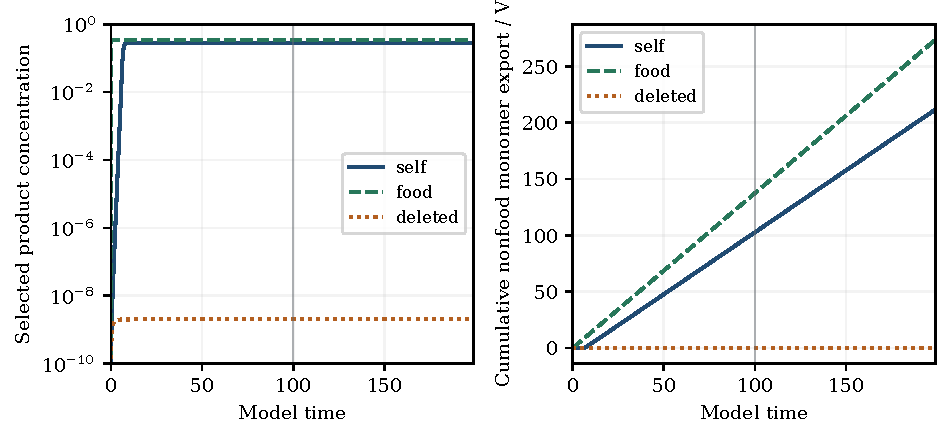
\includegraphics[width=.95\linewidth]{matched.pdf}
\caption{Matched full-catalogue concentration trajectories for the three specified environments. All curves are numerical ODE solutions, not certified count trajectories. The panels separate the selected product from the cumulative collected nonfood mass; the deleted baseline retains positive basal chemistry.}
\label{fig:matched}
\end{figure}

The count-process diagnostic runs the exact stochastic simulation algorithm \cite{gillespie1977exact} with falling-factorial propensities, all channels, the food feed and washout, from the food-only state to the deadline $1$, at $V=100$ for the three environments and at the predeclared second setting $V=200$ for the self environment; each row has $200$ independently seeded clocks, and corresponding intervention rows share seed labels, which does not by itself provide a pathwise monotone coupling. Each path records the first nonfood molecule, the first selected product, the first corridor exit, and the counts. Table~\ref{tab:ssa} separates these observables, which the mission conflates.

\begin{table}[t]
\centering\small
\begin{tabular}{@{}lrrrrrr@{}}
\toprule
Environment & $V$ & Runs & Nonfood by $1$ & Selected by $1$ & Births before exit & Exits by $1$\\
\midrule
Self & 100 & 200 & 0 & 0 & 0 & 5\\
Self & 200 & 200 & 0 & 0 & 0 & 0\\
Food & 100 & 200 & 200 & 200 & 200 & 5\\
Deleted & 100 & 200 & 0 & 0 & 0 & 5\\
\bottomrule
\end{tabular}
\caption{Exact-algorithm count-process startup diagnostics at $n=4$. In the food row every first nonfood molecule is the selected product and appears before time $0.0154$. The five corridor exits at $V=100$ are feed fluctuations crossing $11V$ within one time unit, a finite-count effect absent from the deterministic model; they are retained, not conditioned away. Each path has between $1100$ and $2600$ events.}
\label{tab:ssa}
\end{table}

Two remarks fix what the diagnostic can and cannot show. First, a zero-birth row of $200$ runs has exact two-sided $95\%$ binomial upper endpoint $0.01828$, whereas the analytic ceilings of Theorem~\ref{thm:birth} are $3.2\times10^{-5}$ at $V=100$ and $6.5\times10^{-5}$ at $V=200$: observing no initiation is compatible with the bound but cannot resolve its value, and the $V=200$ row was a prospective prediction that the bound survived, not a measurement of it. Second, the mechanistic distinction is visible without statistics: food catalysis can act at the first event, whereas an absent product cannot catalyze its own first appearance, and at $V=100$ the total basal birth rate is at most $\lambda V=3.2\times10^{-5}$ per unit time, so the food-silent rows had no realistic chance to initiate by the deadline. That is the content of the necessary scale.

\section{Dimensions, interpretation, and scope}\label{sec:units}

An illustrative dimensionalization uses a concentration scale $c_*$ in mol/L, a physical volume $\Omega$ in litres and a residence time $\tau_{\rm res}$:
\begin{equation}\label{eq:dimensions}
 V=N_A\Omega c_*,\qquad t_{\rm phys}=\tau_{\rm res}\,t,\qquad k_{\rm phys}=\frac\kappa{\tau_{\rm res}c_*^{\,m-1}},
\end{equation}
for a dimensionless coefficient $\kappa$ of full molecularity $m$. Forward ligation and reverse cleavage have different molecularities, and an explicit catalyst adds a reactant factor, so equal dimensionless paired coefficients do not have equal dimensional units. At $c_*=1\,\mu$M the necessary $99\%$ startup scale $V=1.43\times10^7$ corresponds to about $23.7$ pL and to an initial food population of $6V\approx8.6\times10^7$ molecules; the envelope scale $2.5\times10^{61}$ at $n=4$ to $4.2\times10^{43}$ L, the direct witness scale $8.97\times10^{50}$ to $1.5\times10^{33}$ L, and the unequal-tolerance scale $5.0\times10^{49}$ to $8.3\times10^{31}$ L. The first number is a necessary condition and not a reactor design; the others demonstrate the conservatism of the concentration-level analysis and not achievable equipment. Taking $\tau_{\rm res}=1$ h gives a $199$-hour mission at dilution rate $1\,\mathrm h^{-1}$; it does not calibrate the reaction coefficients to any chemistry, and there is no experimentally determined mapping from binary words to molecules in this study.

\begin{table}[t]
\centering\small
\begin{tabular}{@{}p{.2\linewidth}p{.38\linewidth}p{.36\linewidth}@{}}
\toprule
Feature & Treatment here & Consequence\\
\midrule
Discrete counts & explicit falling-factorial jump process & first-molecule barriers and demographic noise are represented\\
Reversibility & both directions of every split identity & signed synthesis and reverse losses are accounted for\\
Resources & maintained feed with a finite observed expenditure allowance & finite mission accounting, not an autonomously depleting reservoir\\
Background chemistry & every nonfood row retained in the witness & a full-catalogue statement within the declared source\\
Degradation and waste & uniform washout; no damage or inhibition & selective destruction needs new drift estimates\\
Spatial structure & well mixed; no diffusion or membrane & no transport-limited prediction\\
Product identity & aggregate nonfood export; existential length-four stock & no target-specific activity or purification\\
Thermochemistry & paired dimensionless coefficients & material accounting is not a work or dissipation theorem\\
\bottomrule
\end{tabular}
\caption{What the model includes and omits.}
\label{tab:scope}
\end{table}

Table~\ref{tab:scope} lists the modelling choices. The immediate methodological content is concrete: define the operating task before screening networks, distinguish source occurrence from operating reliability, expose the initiation bottleneck separately from the growth argument, and require compatible material and uncertainty accounts. A physically grounded successor would start from an explicit molecular reaction set with measurable rates and preserve stoichiometry, rate units, catalyst multiplicities, driving species and reservoir conditions; nothing here transfers automatically from binary words to activated oligomers or enzymatic ligation.

\section{Discussion}\label{sec:discussion}

\paragraph{Three requirements, three scales.}
Availability of a productive organization, creation of its first molecules, and execution of a specified task are different requirements with different quantitative statements. Availability is a source event of probability $224p_{a,n}+o(p_{a,n})$ for the productive singletons and $\theta>0$ for RAFs in general. Initiation in a food-silent environment is a first-passage event with hazard at most $\lambda V$, hence a necessary scale $V\ge\log(1/\eta)/\lambda$. Execution, on one uninterrupted trajectory with stock at three times and export in two windows, has probability of order $p_{a,n}$ at a sufficient scale, and conditioning on it selects a single productive incidence. Treating ``a RAF exists'' as an operating prediction collapses these distinctions.

\paragraph{What the two-window event adds.}
The event demands two actual output windows and endpoint stock on the same trajectory while accounting for the gross supply. The proof handles this without a restart theorem: the interval estimate \eqref{eq:interval} is stated for an arbitrary actual interval and telescopes across the middle observation time, and the six noise controls are imposed once on the whole horizon. This is weaker than uniform restart from every state in the stock region and weaker than indefinite operation, and it is stated as such. The material identity shows that the exported mass is net internal synthesis, since the reactor starts with no nonfood inventory.

\paragraph{Where the constants come from.}
The loss coefficients $23$ and $25$ are the corridor bound $\sum_zx_z\le11$ counted in two input positions plus the number of cleavage positions; the drift constant $2$ is $4\cdot\tfrac34-1$; the endpoint constant $54$ is the range of $\log x-4H$ between the stock floor and the mass cap; and the window length $79$ is the least duration at which \eqref{eq:margin} exceeds $\tfrac1{10}$. None of these sets the count scale. The scale is set by the absolute product tolerance $\floorstock/100$, entering squared in $c$; Proposition~\ref{prop:scales} shows exactly how far the estimate can be improved by choosing tolerances and where a new inequality is required.

\paragraph{Open problems.}
(1) A sufficient count scale within reach of the necessary one, through a seed-to-established-stock comparison with relative rather than absolute error. (2) A finite converse that weighs occupied catalysts on the actual path under the size-biased row law, replacing the count of potential incidences; this is also what singleton dominance for $1<a<2$ would need. (3) The relative operational weights of the $224$ productive labels, that is, the limits of the environment-averaged conditional success probabilities identified in \cite{diffuse2026}. (4) A restart theorem from an arbitrary state in the stock region, and more than two windows. (5) A thermochemically consistent source in which the exported mass can be related to work and dissipation \cite{rao2016nonequilibrium}. None of these alters the finite statements proved here.

\paragraph{Data and code availability.}
\RepositoryNote{} The editable source package contains the paper, the bibliography, the figure data and scripts, the exact-arithmetic replay of every printed number, the raw simulation records, and the two strict verification receipts (Appendix~\ref{app:formal}).

\appendix

\section{Explicit constants and source formulas}\label{app:constants}

\paragraph{The common-tolerance choice.}
With $d_N=\dots=d_B=d$ and $V\ge2n/d$, the margins \eqref{eq:margins} hold for $n\ge4$ because $n/V\le d/2$ and $2/V\le d/2$, and $d+d/2\le\tfrac18,\tfrac1{80},10^{-5},\tfrac1{3\times10^{20}},\tfrac1{40},1$ respectively; the last inequality is the only one with slack of less than a factor two, since $d=\tfrac12\cdot\tfrac1{3\times10^{20}}$. Every exponent is then at least $cV/n$, and the six coefficients sum to $24$. At $V=V_*(n)$, $\delta_{n,V}=24e^{-48}\approx3.4\times10^{-20}$ for $n=4$ and decreases with $n$.

\paragraph{Source moments.}
The moments \eqref{eq:moments} are evaluated as $\sum_{k=1}^{R-1}k^{-s}=\zeta(s)-\zeta(s,R)$ for $s\ne1$, with $\zeta(s,R)$ the Hurwitz zeta function, and as the harmonic number for $s=1$; this is how the values in Figure~\ref{fig:exponent} and the checks of the replay script are computed. At $a_n=2-2/n$ the normalized first moment satisfies $\EE D/n\to(1-e^{2\log2})/[-2\zeta(2)]=9/\pi^2$, the profile of the formal development at the parameter $-2$, and with $X_n\sim2\cdot2^n$, $R_n\sim2n2^n$ this is \eqref{eq:rarity}. Numerically $2^np_n$ equals $2.604$, $1.455$, $0.928$, $0.693$ and $0.580$ at $n=4,8,16,32,64$; the approach to $0.456$ is slow, of relative order $1/n$.

\paragraph{The conditional sampler.}
Conditioning a row on containing one specified incidence changes the degree law to $\PP(D=d\mid r\in C_z)=d\,\PP(D=d)/\EE D$, after which the remaining $d-1$ coordinates are uniform. For $k$ required and $\ell$ forbidden distinct coordinates the likelihood multiplier is $(d)_k(R_n-d)_\ell/(R_n)_{k+\ell}$. At $n=4$ the cap atom has probability about $0.09$ unconditionally and about $0.56$ after requiring one incidence. Planting an incidence into an unconditioned row is therefore not an exact conditional sampler, and any finite converse that weighs occupied catalysts must use this law.

\paragraph{Exact values of the finite obstruction.}
At $n=4$, $a=\tfrac32$: $X_4=30$, $p_0=1/\zeta(\tfrac32)=0.3828$, $p_1=2^{-3/2}p_0$, and the complement in \eqref{eq:finiteobstruction} is $p_0^{30}+30p_1p_0^{29}=10^{-11.446}$.

\section{Formal scope and reproducibility}\label{app:formal}

The Lean development is a single project pinned to \texttt{leanprover/lean4:v4.30.0} with a pinned Mathlib manifest; the reactor namespace \lean{RandomViability} imports the source namespace \lean{PowerLawSmallRAF}, and both use one configuration weight for the capped, shifted Zipf sampler. The core declaration is
\begin{center}\small\lean{RandomViability.c6_two_window_resolution}\end{center}
in \path{proofs/RepeatedFunction/C6Resolution.lean}. Its strict receipt records exit code zero, warnings treated as errors, empty compiler output, $425$ dependency sources with their SHA-256 hashes, the pinned toolchain and manifest, and the transitive axioms \texttt{propext}, \texttt{Classical.choice} and \texttt{Quot.sound} only; the source hash of the root is \texttt{a18c3766\ldots3060}. The declaration asserts, for every integer volume sequence $V_n\ge V_*(n)$: the finite bracket $0<\text{lower}\le S\le\text{upper}$ for every $n\ge4$ and $a>1$, with the lower bound $e_a^6p_{a,n}(1-24e^{-cV/n})$ and the upper bound $15480p_{a,n}+\bar r$; the eventual bounds $\tfrac12(6/\pi^2)^6p_n\le S_n\le15481p_n$ at $a_n=2-2/n$; the eventual posterior bound $\tfrac12(6/\pi^2)^6/15481$ for the seed class; the vanishing conditional probability of no productive singleton; and, for every environment and mark configuration, the almost-sure signed synthesis $J(199)>V/5$ on the mission. Its event is exactly Definition~\ref{def:event} (\lean{twoWindowMission}), including stock at time $1$.

A second strict receipt, for \path{proofs/RepeatedFunction/PublicationBundle.lean}, checks \lean{ProductiveCensus.lean} and \lean{StartupNecessary.lean}: the count $224$ at cap four by kernel evaluation, the injection of the labels of every catalogue into cap four, the equivalence of the productive predicate with the union event, the food-pair maximum $121/3$, the rate consequence, the finite-kernel survival induction, the logarithmic necessary-scale inequality and the scalar material-ratio inequality; $428$ dependency entries, empty compiler output, the same three axioms. Table~\ref{tab:formal} maps the statements of this paper to their evidence.

\begin{center}\small
\begin{tabular}{@{}>{\raggedright\arraybackslash}p{.34\linewidth}>{\raggedright\arraybackslash}p{.62\linewidth}@{}}
\toprule
Statement & Evidence\\
\midrule
Lemma~\ref{lem:envelopes} (loss envelopes) & \lean{physical_food_drift_bound}, \lean{physical_product_drift_bound}; derivation in the text\\
Lemma~\ref{lem:potential} & \lean{collectivePotential} and its derivative lemma; proof in the text\\
Lemmas~\ref{lem:mass}, \ref{lem:startup} & \lean{physical_mass_localization}, \lean{physical_startup_product_from_noise}\\
Lemmas~\ref{lem:holding}, \ref{lem:endpoint} & \lean{physical_holding_potential_gain}, \lean{physical_potential_endpoint_penalty}\\
Proposition~\ref{prop:interval}, Corollary~\ref{cor:export} & \lean{physical_interval_potential_gain}, \lean{physical_interval_mass_from_noise}, \lean{physical_interval_export_lower}, \lean{interval_export_margin}\\
Lemma~\ref{lem:six} and \eqref{eq:uniform} & \lean{physical_two_window_failure_tail}, \lean{physical_two_window_uniform_tail}, \lean{concrete_two_window_success_lower}\\
Source averaging \eqref{eq:lower} & \lean{source_food_silent_seed_mass}, \lean{fully_averaged_two_window_lower}\\
Lemma~\ref{lem:exclusion} & \lean{physical_output_upper_at_most_one_local} (companion \cite{diffuse2026})\\
Lemma~\ref{lem:census}, count and predicate & \lean{productive_labels_four}, \lean{productive_labels_card_le}, \lean{productive_union_iff}; union bound \eqref{eq:census} conventional\\
\eqref{eq:upper}, \eqref{eq:bad} with $15480$ & \lean{averaged_mission_finite_upper}, \lean{two_window_finite_source_resolution}\\
Lemma~\ref{lem:material} & \lean{actual_net_synthesis_identity}, \lean{food_only_mission_net_synthesis}, \lean{mission_material_recovery}\\
Theorem~\ref{thm:limits} & limits \eqref{eq:sourcelimits} formal; eventual bounds with $\gamma/2$, $15481$ in the root; full constants conventional\\
Section~\ref{sec:transfers} & \lean{two_local_incidence_mass_div_incidence_tendsto_zero}, \lean{source_RAF_probability_tendsto}; transfers conventional\\
Theorem~\ref{thm:birth} & \lean{food_pair_birth_bound}, \lean{startup_intensity_bound}, \lean{startup_survival_lower}, \lean{startup_necessary_scale}; stopped-generator identification and Poisson mixture conventional\\
Theorem~\ref{thm:robust} & first-moment limit along families \lean{windowZipfMean_source_window_normalized}; all else conventional\\
Proposition~\ref{prop:scales} & conventional evaluation of Lemma~\ref{lem:six}\\
Sections~\ref{sec:example}, \ref{sec:units} & numerical illustration; no proof premise\\
\bottomrule
\end{tabular}
\captionof{table}{Claims and their evidence. Lean names live in \texttt{proofs/RandomViability/}, \texttt{proofs/RepeatedFunction/} and \texttt{proofs/PowerLawSmallRAF/}.}
\label{tab:formal}
\end{center}

\paragraph{Conventional proofs.}
The union bound that replaces $15480$ by $224$, the limiting constants of Theorem~\ref{thm:limits}, the screening formula, the reliability inequality, the four transfers, the stopped-generator identification and Poisson mixture in Theorem~\ref{thm:birth}, Theorem~\ref{thm:robust} except its first-moment limit, and Proposition~\ref{prop:scales} are proved in the text and are not additional terminal Lean exports. The finite-kernel induction alone does not certify that a particular physical generator meets its hypotheses; that identification is the explicit argument of Section~\ref{sec:startup}.

\paragraph{Reproduction.}
The exact-arithmetic script \texttt{check\_paper.py} distributed with the source replays every printed number: the catalogue counts and the census, the noise constants and margins, the drift and endpoint algebra, the window margins and the threshold $79$, the material ratio, the hazard and the necessary scale, the source moments and every asymptotic formula of Theorem~\ref{thm:robust} against exact Hurwitz-zeta evaluations, the unequal-tolerance thresholds, the finite obstruction, the dimensional conversions, and the numerical tables from the retained raw records; it also checks the two receipts for verification status, dependency counts and axioms. The figure script regenerates the four figures from the retained data. The simulation script, its full-catalogue definitions, and the raw per-path records are included for provenance; the production run used seeds $91000$--$91199$, a single numerical worker, and a checked event cap that no path reached. Formal verification uses the repository bridge, which pins the Mathlib working directory, treats warnings as errors and writes the receipts; no dependency update is performed.

\bibliographystyle{plainnat}
\bibliography{refs}

\end{document}
